\documentclass[11pt,a4paper]{article}

\usepackage[utf8]{inputenc}
\usepackage[francais]{babel}
\usepackage[T1]{fontenc}
\usepackage{amsmath}
\usepackage{amsfonts}
\usepackage{amssymb}
\usepackage[colorlinks=false]{hyperref} % liens dans le sommaire
% \usepackage[top = 2.54cm, bottom = 2.54cm, left = 2.54cm, right = 2.54cm]{geometry}
\usepackage[top = 2cm, bottom = 2cm, left = 2cm, right = 2cm]{geometry}
\usepackage{graphicx}
\usepackage{caption}
\hypersetup{colorlinks, linkcolor = black, citecolor = black} % enlève couleur des liens
\usepackage{hyperref}
\usepackage{color}
\frenchbsetup{StandardLists=true}
\usepackage{float}
\usepackage{fancyhdr}
\usepackage{mathtools}
\pagestyle{fancy}

\newcommand{\dx}[1]{\dfrac{\partial #1}{\partial x}}
\newcommand{\norm}[1]{\big|\big|#1\big|\big|}
\newcommand{\question}[2]{\paragraph{Question #1 --}\hspace{-7pt}\textit{#2} \\}
\newcommand{\questions}[2]{\paragraph{Questions #1 --}\hspace{-7pt}\textit{#2} \\}
\newcommand{\tphi}{\widetilde{\Phi}}
\newcommand{\intsigma}{\widetilde{\Sigma}}
\newcommand{\F}{\mathcal{F}}
\newcommand{\Qt}{\widetilde{Q}}
\newcommand{\Phit}{\widetilde{\Phi}}
%\makeatletter \def\input@path{{Graphics/}} \makeatother

\begin{document}

\begin{titlepage}
  ~\vspace{90pt}
  \centering \bfseries

  \huge Rapport de TP \\AMS302

  \vspace{50pt}
  \rule{0.5\textwidth}{1pt}
  \vspace{50pt}

  \Huge Solveur Déterministe \\ pour le transport de particules neutres

  \vspace{50pt}
  \rule{0.5\textwidth}{1pt}

  \vspace{50pt}
  \huge {\itshape Benoît Sohet \\ \& \\ Aurélien Valade}

  \vfill
  \begin{tabular}{cc}
    \begin{minipage}{.49\textwidth}
      \centering
      %\includegraphics[height=0.1\textheight]{logo_ups}
    \end{minipage}
    &
      \begin{minipage}{.49\textwidth}
        \centering
        %\includegraphics[height=0.1\textheight]{logo_ensta}
      \end{minipage}
  \end{tabular}

\end{titlepage}

\newpage

\section*{Introduction}

Dans ce TP on cherche à résoudre le problème différentiel suivant 
\begin{equation}
  \label{eq:principal}
  \begin{cases}
    \mu \dx{\Phi}(x, \mu) + \Sigma_t(x) \Phi(x, \mu) =
    \dfrac{1}{2} \Sigma_s(x) \int_1^{-1} \Phi(x, \mu') d\mu' + S(x, \mu) & \forall (x, \mu) \in [0,1]\times[-1,1]  \medskip\\ 
    \mu n(x) < 0  & \forall (x, \mu) \in \{0,1\}\times[-1,1] 
  \end{cases}
\end{equation}

\begin{itemize}
\item $\Phi(x, \mu)$ le flux neutronique
\item $\Sigma_t$ la section efficace totale 
\item $n(x)$ la normale sortante : $n(0) = -1, ~ n(1) = 1$
\end{itemize}

On fixe pour cela deux types de conditions aux limites 
\begin{itemize}
\item Flux entrant à gauche
  \begin{equation}
    \begin{cases}
      \Phi^{-} (0, \mu) = \frac{1}{\mu}  ~~~ \forall \mu \in [0,1]\\
      \Phi^{-} (1, \mu) = 0 ~~~ \forall \mu \in [-1,0]
    \end{cases}
  \end{equation}
\item Source nulle ou unitaire
  \begin{align}
    S(x) &= 0 ~~~ \forall x \in [0,1] \\
    S(x) &= 1 ~~~ \forall x \in [0,1] 
  \end{align}
\end{itemize}	

On utilisera dans la suite l'erreur pour une fonction $f$ et son approximation $\tilde{f}$ : 
\begin{equation}
  e_{L^2}(f, \tilde{f}) = \frac{\norm{f-\tilde{f}}_{L_2}}{\norm{f}_{L_2}}
\end{equation}

\emph{L'utilisation des codes nécessite gnuplot ainsi qu'un système d'exploitation respectant la norme POSIX.}

\section{Matériau purement absorbant}

\subsection{Matériau homogène - courant entrant unitaire}

\question{9.1}{Rappeler la solution analytique à ce problème avec source nulle et flux entrant à gauche, et un matériau purement absorbant et homogène.}

L'équation à résoudre s'écrit alors :
\begin{equation}
  \begin{cases}
    \mu \dx{\Phi}(x, \mu) + \Sigma_a \Phi(x, \mu) = 0 & \forall (x, \mu) \in [0,1]\times[-1,1]  \medskip\\ 
    \Phi(0,\mu) = \frac{1}{\mu} & \forall \mu \in [0,1] \medskip\\
    \Phi(1,\mu) = 0 & \forall \mu \in [-1,0]
  \end{cases}
  \label{eq:pasdiff}
\end{equation}

La solution est donc :
\begin{equation}
 \Phi(x, \mu) = A(\mu) e^{-\frac{\Sigma_a}{\mu}x} ,
\end{equation}

avec $A(\mu)$ qui vérifie les conditions initiales :
\begin{equation}
 A(\mu) = 
 \begin{cases}
  \frac{1}{\mu} & \text{si } \mu \in [0,1] \\
  0             & \text{si } \mu \in [-1,0] .
 \end{cases}
\end{equation}

On peut remarquer que l'on retrouve exactement la même solution que si l'on avait imposé un flux entrant nul des deux côtés, et une source sous forme de dirac en 0 lorsque $\mu>0$.

\question{9.2}{Implémenter un solveur déterministe permettant d'évaluer le flux neutronique en chaque point de la géométrie. Ce solveur sera basé sur la méthode ``diamant'' pour la discrétisation spatiale.} 

\paragraph{Notations :} On note par $(x_i)$ la segmentation choisie pour $[0,1]$, $I_i = [x_i,x_{i+1}]$ et $\delta_i = x_{i+1} - x_i$.
On peut alors écrire $\phi_i( \mu) = \phi(x_i,\mu)$.
La méthode ``diamant'' fait l'hypothèse suivante :

\begin{equation}
 \forall (\mu,x) \in [-1,1]\times I_i, \quad \phi(x,\mu) \simeq \frac{\phi_i(\mu) + \phi_{i+1}(\mu)}{2} .
\end{equation}
Pour simplifier les expressions suivantes, on se fixe un $\mu \in  [-1,1]$ et on écrit directement $\phi_i(\mu) = \phi_i$.
De là, l'équation~\ref{eq:pasdiff} devient (on rajoute un terme source $S$ pour ne pas avoir à refaire les calculs pour la prochaine question) :

\begin{align}
& \mu \frac{\phi_{i+1}-\phi_i}{\Delta_i} + \Sigma_t \frac{\phi_{i+1}+\phi_i}{2} = S\\
\Leftrightarrow \quad
& 2 \mu (\phi_{i+1}- \phi_i) + \Delta_i \Sigma_t (\phi_{i+1}+\phi_i) = 2 \Delta_i S\\
\Leftrightarrow \quad
& \eta^+ \phi_{i+1} - \eta^- \phi_i = 2 \Delta_i S
&& 	\text{avec } \eta^{\pm} = 2 \mu \pm \Delta_i \Sigma_t .
\end{align}

Or, suivant le signe de $\mu$, on n'isolera pas le même terme dans cette équation.
En effet, si $\mu>0$, les conditions de flux entrant ne donnent une information qu'en $x=0$ : il faut donc utiliser cette relation récurrente afin d'avoir $\phi_{i+1}$ à partir de $\phi_i$, ce qui donne :
\begin{equation}
 \phi_{i+1} = \frac{\eta^- \phi_i + 2 \Delta_i S}{\eta^+}
 \label{eq:recu}
\end{equation}

Et inversement lorsque $\mu<0$.
De plus on remarque que :
\begin{equation}
 \frac{\eta^+}{\eta^-} = \frac{- \eta^+}{-\eta^-} = \frac{-2 \mu - \Delta_i \Sigma_t}{-2 \mu + \Delta_i \Sigma_t} = \frac{2 |\mu| - \Delta_i \Sigma_t}{2 |\mu| + \Delta_i \Sigma_t} ,
\end{equation}

donc si l'on change la définition des $\eta$ en $\eta^{\pm} = 2|\mu| \pm \Delta_i \Sigma_t$, on retrouve pour $\mu<0$ la même formulation~\ref{eq:recu} que pour $\mu>0$ :
\begin{equation}
 \phi_i = \frac{\eta^- \phi_{i+1} + 2 \Delta_i S}{\eta^+} .
\end{equation}
Il faut simplement faire attention à bien retourner le vecteur $(\phi_i)$.

\subsection{Matériau homogène - source uniforme}

\question{10}{Reprendre la démarche de la question 9 pour ces nouvelles conditions. On veillera à ce que les fonctionnalités
 ajoutées dans le solveur pour le traitement du terme source restent compatibles avec le traitement du flux entrant imposé nécessaire pour la question 9.}

 \subsection{Matériau non homogène - courant entrant unitaire}
 
 On se place maintenant dans le cas d'une source nulle et de conditions de flux entrant imposé, pour un matériau non homogène :
\begin{equation}
  \Sigma_a =
  \begin{cases}
    1 &\mbox{si } x<0.3 \\
    3 &\mbox{si } 0.3<x<0.7 \\
    1 &\mbox{si } 0.7<x \\
  \end{cases}
\end{equation}

\question{11}{Reprendre la démarche de la question 9 pour ces nouvelles conditions.
On s'attachera à ce que les fonctionnalités ajoutées pour le traitement de sections efficaces variables restent compatibles avec le reste du solveur tel que développé dans les questions précédentes.}

\section{Matériau diffusant}

\question{12}{Reprendre la démarche de la question 9 pour traiter ce problème de diffusion.
Le solveur utilisera la méthode des ordonnées discrètes ($S_N$) pour traiter la variable angulaire $\mu$.
Il n'y a pas de solution analytique dans ce cas ; on s'attachera donc tout particulièrement à la vérification du solveur déterministe par comparaison aux résultats donnés par le solveur Monte Carlo développé au TP1.}

Voici la structure générale du code (prenant en compte la diffusion aussi, présentée pour $\mu>0$), pour une discrétisation en $N_x$ points en espace et $N_{\mu}$ en direction.

\begin{itemize}
\item Récupération et vérification des arguments
\item Allocation de la mémoire
\item $Q_1 = S, \quad Q_0 = Q + \varepsilon_s +1$
\item[\textcolor{red}{\textbullet}] Tant que $\norm{Q_1 - Q_0}>\varepsilon_s$
  \setlength\itemindent{35pt}
\item $\Phit=0~[N_x]$
\item[\textcolor{red}{\textbullet}] Pour $k\in[1,N_{\mu}]$
  \setlength\itemindent{70pt}
\item $\Phi^- = 0$
\item[\textcolor{red}{\textbullet}] Pour $i\in[1, N_x-1]$
  \setlength\itemindent{105pt}
\item $\Phi^+ = \frac{\eta^- \Phi^- + 2 \Delta_i S}{\eta^+}$
\item $\Phit_i =  \Phit_i + \frac{1}{2} w_k (\Phi^+ + \Phi^-)$
\item $\Phi^- = \Phi^+$
  \setlength\itemindent{70pt}
\item[\textcolor{red}{\textbullet}] Fin pour $i$
   \setlength\itemindent{35pt}
\item[\textcolor{red}{\textbullet}] Fin pour $k$ 
\item $Q_0 = Q_1$
\item $Q_1 = S + \frac{\Sigma_s}{2} \Phit$
   \setlength\itemindent{0pt}
\item[\textcolor{red}{\textbullet}] Fin tant que  
\end{itemize}
 
 \section{Limite de diffusion}
 
 Nous nous intéressons maintenant au cas de matériaux très diffusants et peu absorbants, correspondants au problème suivant, caractérisé par un paramètre $\epsilon$ :
  \begin{align}
   &\Sigma_a(x) = \epsilon \sigma_a\\
   &\Sigma_t(x) = \frac{\sigma_t}{\epsilon}\\
   &\Sigma_s(x) = \frac{\sigma_t}{\epsilon} - \epsilon \sigma_a
  \end{align}
 assorti d'une source uniforme $S = \epsilon$ et des conditions aux limites de flux entrant nul.
 On note $\Phi_\epsilon$ la solution du problème\ref{eq:principal} dans ces conditions, et $\Phit_\epsilon$ le flux scalaire associé :
 \begin{equation}
  \forall x\in [0,1], \quad \Phit_\epsilon = \frac{1}{2} \int_{-1}^1 \Phi_\epsilon(x,\mu) d\mu .
 \end{equation}
 
\question{13.1}{Trouver l'équation vérifiée par $\Phi_\epsilon$ lorsque $\epsilon$ tend vers 0.}

Selon ces hypothèses, l'équation se réécrit alors :
\begin{equation}
 \mu \frac{\partial \Phi_\epsilon}{\partial x} + \frac{\sigma_t}{\epsilon} \Phi_\epsilon =  \epsilon + \left(\frac{\sigma_t}{\epsilon} - \epsilon \sigma_a\right) \Phit_\epsilon .
 \label{eq:eps}
\end{equation}

La présence du $\frac{1}{\epsilon}$ nous invite à supposer que l'on peut écrire :
\begin{equation}
 \Phi_\epsilon = \Phi_0 + \epsilon\Phi_1 + \epsilon^2 \Phi_2 + ... ,
\end{equation}
et de même pour $\Phit_\epsilon$.
Puis, on pourra ensuite dissocier les termes de l'équation\ref{eq:eps} selon devant quelle puissance de $\epsilon$ ils se trouvent : chacun devra être nul.
Le terme en facteur de $\frac{1}{\epsilon}$ est :
\begin{equation}
 \sigma_t (\Phi_0(x,\mu) - \Phit_0(x)) = 0 \quad \Leftrightarrow \quad \Phi_0(x,\mu) = \Phit_0(x) \quad \forall \mu \in [-1,1]
\end{equation}
Nous n'utiliserons donc plus que $\Phi_0(x)$.

Regardons ensuite tout d'abord le terme devant la puissance $\epsilon^1$, divisé par 2, et que l'on intègre sur $\mu$ entre -1 et 1 :

\begin{equation}
 \frac{1}{2}\int_{-1}^1 \left[ \mu \dx{\Phi_1} + \sigma_t (\Phi_2(x,\mu) - \Phit_2(x)) + \sigma_a \Phit_0(x) -1 \right] d\mu
 = \sigma_a \Phi_0(x) -1 + \textcolor{red}{\frac{1}{2}\int_{-1}^1  \mu \dx{\Phi_1} d\mu} \quad = 0.
\end{equation}
Le dernier terme de droite donne l'idée d'intégrer le terme devant le facteur $\epsilon^0$ en premier lieu multiplié par $\mu$ :
\begin{equation}
 \frac{1}{2} \int_{-1}^1 \mu^2 \frac{d\Phi_0}{dx} d\mu + \sigma_t \times \frac{1}{2}\int_{-1}^1  \mu \Phi_1 d\mu - 0
 \quad = \quad \frac{1}{3} \frac{d\Phi_0}{dx} + \textcolor{red}{\sigma_t \times \frac{1}{2}\int_{-1}^1  \mu \Phi_1 d\mu}
 \quad = \quad 0
\end{equation}

On voit qu'il reste une chose supplémentaire à faire, à savoir dériver la dernière équation par rapport à $x$, ce qui nous laisse :

\begin{equation}
- \frac{1}{3 \sigma_t} \frac{d^2 \Phi_0}{d x^2}(x) + \sigma_a\Phi_0(x) = 1 .
\end{equation}

C'est cette équation que vérifie $\Phi_\epsilon$ lorsque $\epsilon$ tend vers 0, car $\lim\limits_{\epsilon \rightarrow 0} \Phi_\epsilon = \Phi_0$.

\question{13.2}{Dans le cas où on prend $\sigma_a = 0$ et $\sigma_t = 1$, trouver la limite de $\Phi_\epsilon$ lorsque $\epsilon$ tend vers 0.}

D'après la question précédente, dans ce cas l'équation vérifiée est :
\begin{equation}
- \frac{1}{3} \frac{d^2 \Phi_0}{d x^2}(x) = 1 .
\end{equation}
Les solutions de cette équation sont de la forme $\Phi_0(x) = -\frac{3}{2}x^2 + a x +b$, avec $a$ et $b$ des constantes à déterminer avec les conditions aux limites : on sait que $\Phi_0(0,\mu >0) = \Phi_0(1,\mu <0) = 0$.
Or, $\Phi_0(x,\mu) = \Phi_0(x) \quad \forall \mu \in [-1,1]$, donc cela nous permet de conclure sur $\Phi_0(x) = \frac{3}{2}x(1-x)$.

\questions{14 et 16}{Dans ce dernier cas, trouver la solution $\Phit_\epsilon$ avec votre code pour $\epsilon = 1, 0.1, 0.01$. Donner le nombre d'itérations de la source itérée pour chaque valeur de $\epsilon$. Que peut-on constater ?}

Ci-dessous se trouve un tableau donnant le nombre d'itérations nécessaires à la convergence ($\norm{Q_1 - Q_0}>10^{-3}$, voir l'algorithme de la question 12), pour chaque valeur de $\epsilon$, et avec ou sans accélération par diffusion synthétique.
Une expérience n'aura pas convergé si la condition de convergence n'est toujours pas remplie au bout de 10000 itérations (équivalant à environ 40s).
Dans ce cas, ce ne sera pas le nombre d'itérations mais la valeur de $\norm{Q_1 - Q_0}$ qui sera présentée dans le tableau.

\begin{tabular}{|c|c|c|c|}
  \hline
  $\epsilon = $ & 1 & 0.1 & 0.01 \\
  \hline\hline
  \textit{sans} DSA & 1.1 & 1.2 & 1.3 \\
  \textit{avec} DSA & 2.1 & 2.2 & 2.3 \\
  \hline
\end{tabular}

%% GNUPLOT: LaTeX picture with Postscript
\begingroup
  \makeatletter
  \providecommand\color[2][]{%
    \GenericError{(gnuplot) \space\space\space\@spaces}{%
      Package color not loaded in conjunction with
      terminal option `colourtext'%
    }{See the gnuplot documentation for explanation.%
    }{Either use 'blacktext' in gnuplot or load the package
      color.sty in LaTeX.}%
    \renewcommand\color[2][]{}%
  }%
  \providecommand\includegraphics[2][]{%
    \GenericError{(gnuplot) \space\space\space\@spaces}{%
      Package graphicx or graphics not loaded%
    }{See the gnuplot documentation for explanation.%
    }{The gnuplot epslatex terminal needs graphicx.sty or graphics.sty.}%
    \renewcommand\includegraphics[2][]{}%
  }%
  \providecommand\rotatebox[2]{#2}%
  \@ifundefined{ifGPcolor}{%
    \newif\ifGPcolor
    \GPcolorfalse
  }{}%
  \@ifundefined{ifGPblacktext}{%
    \newif\ifGPblacktext
    \GPblacktexttrue
  }{}%
  % define a \g@addto@macro without @ in the name:
  \let\gplgaddtomacro\g@addto@macro
  % define empty templates for all commands taking text:
  \gdef\gplbacktext{}%
  \gdef\gplfronttext{}%
  \makeatother
  \ifGPblacktext
    % no textcolor at all
    \def\colorrgb#1{}%
    \def\colorgray#1{}%
  \else
    % gray or color?
    \ifGPcolor
      \def\colorrgb#1{\color[rgb]{#1}}%
      \def\colorgray#1{\color[gray]{#1}}%
      \expandafter\def\csname LTw\endcsname{\color{white}}%
      \expandafter\def\csname LTb\endcsname{\color{black}}%
      \expandafter\def\csname LTa\endcsname{\color{black}}%
      \expandafter\def\csname LT0\endcsname{\color[rgb]{1,0,0}}%
      \expandafter\def\csname LT1\endcsname{\color[rgb]{0,1,0}}%
      \expandafter\def\csname LT2\endcsname{\color[rgb]{0,0,1}}%
      \expandafter\def\csname LT3\endcsname{\color[rgb]{1,0,1}}%
      \expandafter\def\csname LT4\endcsname{\color[rgb]{0,1,1}}%
      \expandafter\def\csname LT5\endcsname{\color[rgb]{1,1,0}}%
      \expandafter\def\csname LT6\endcsname{\color[rgb]{0,0,0}}%
      \expandafter\def\csname LT7\endcsname{\color[rgb]{1,0.3,0}}%
      \expandafter\def\csname LT8\endcsname{\color[rgb]{0.5,0.5,0.5}}%
    \else
      % gray
      \def\colorrgb#1{\color{black}}%
      \def\colorgray#1{\color[gray]{#1}}%
      \expandafter\def\csname LTw\endcsname{\color{white}}%
      \expandafter\def\csname LTb\endcsname{\color{black}}%
      \expandafter\def\csname LTa\endcsname{\color{black}}%
      \expandafter\def\csname LT0\endcsname{\color{black}}%
      \expandafter\def\csname LT1\endcsname{\color{black}}%
      \expandafter\def\csname LT2\endcsname{\color{black}}%
      \expandafter\def\csname LT3\endcsname{\color{black}}%
      \expandafter\def\csname LT4\endcsname{\color{black}}%
      \expandafter\def\csname LT5\endcsname{\color{black}}%
      \expandafter\def\csname LT6\endcsname{\color{black}}%
      \expandafter\def\csname LT7\endcsname{\color{black}}%
      \expandafter\def\csname LT8\endcsname{\color{black}}%
    \fi
  \fi
    \setlength{\unitlength}{0.0500bp}%
    \ifx\gptboxheight\undefined%
      \newlength{\gptboxheight}%
      \newlength{\gptboxwidth}%
      \newsavebox{\gptboxtext}%
    \fi%
    \setlength{\fboxrule}{0.5pt}%
    \setlength{\fboxsep}{1pt}%
\begin{picture}(7200.00,5040.00)%
    \gplgaddtomacro\gplbacktext{%
      \csname LTb\endcsname%%
      \put(814,704){\makebox(0,0)[r]{\strut{}$0$}}%
      \put(814,1218){\makebox(0,0)[r]{\strut{}$0.5$}}%
      \put(814,1733){\makebox(0,0)[r]{\strut{}$1$}}%
      \put(814,2247){\makebox(0,0)[r]{\strut{}$1.5$}}%
      \put(814,2762){\makebox(0,0)[r]{\strut{}$2$}}%
      \put(814,3276){\makebox(0,0)[r]{\strut{}$2.5$}}%
      \put(814,3790){\makebox(0,0)[r]{\strut{}$3$}}%
      \put(814,4305){\makebox(0,0)[r]{\strut{}$3.5$}}%
      \put(814,4819){\makebox(0,0)[r]{\strut{}$4$}}%
      \put(946,484){\makebox(0,0){\strut{}$0$}}%
      \put(2117,484){\makebox(0,0){\strut{}$0.2$}}%
      \put(3289,484){\makebox(0,0){\strut{}$0.4$}}%
      \put(4460,484){\makebox(0,0){\strut{}$0.6$}}%
      \put(5632,484){\makebox(0,0){\strut{}$0.8$}}%
      \put(6803,484){\makebox(0,0){\strut{}$1$}}%
    }%
    \gplgaddtomacro\gplfronttext{%
      \csname LTb\endcsname%%
      \put(198,2761){\rotatebox{-270}{\makebox(0,0){\strut{}$Phi(x, mu)$}}}%
      \put(3874,154){\makebox(0,0){\strut{}$x}}%
      \csname LTb\endcsname%%
      \put(5816,4646){\makebox(0,0)[r]{\strut{}$N_{\mu}$=2}}%
      \csname LTb\endcsname%%
      \put(5816,4426){\makebox(0,0)[r]{\strut{}$N_{\mu}$=4}}%
      \csname LTb\endcsname%%
      \put(5816,4206){\makebox(0,0)[r]{\strut{}$N_{\mu}$=6}}%
      \csname LTb\endcsname%%
      \put(5816,3986){\makebox(0,0)[r]{\strut{}$N_{\mu}$=8}}%
      \csname LTb\endcsname%%
      \put(5816,3766){\makebox(0,0)[r]{\strut{}$N_{\mu}$=10}}%
      \csname LTb\endcsname%%
      \put(5816,3546){\makebox(0,0)[r]{\strut{}$N_{\mu}$=12}}%
      \csname LTb\endcsname%%
      \put(5816,3326){\makebox(0,0)[r]{\strut{}$N_{\mu}$=14}}%
      \csname LTb\endcsname%%
      \put(5816,3106){\makebox(0,0)[r]{\strut{}$N_{\mu}$=16}}%
    }%
    \gplbacktext
    \put(0,0){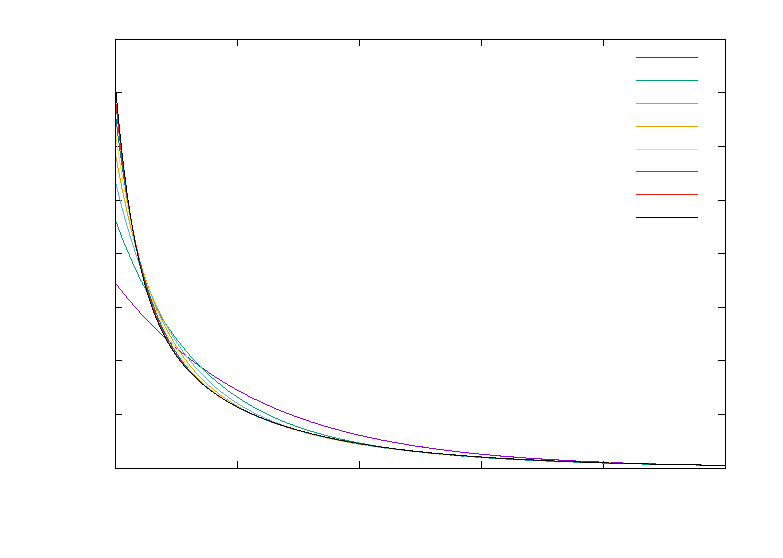
\includegraphics{.\loop_nb_pts_mu_delta.aux}}%
    \gplfronttext
  \end{picture}%
\endgroup

%% GNUPLOT: LaTeX picture with Postscript
\begingroup
  \makeatletter
  \providecommand\color[2][]{%
    \GenericError{(gnuplot) \space\space\space\@spaces}{%
      Package color not loaded in conjunction with
      terminal option `colourtext'%
    }{See the gnuplot documentation for explanation.%
    }{Either use 'blacktext' in gnuplot or load the package
      color.sty in LaTeX.}%
    \renewcommand\color[2][]{}%
  }%
  \providecommand\includegraphics[2][]{%
    \GenericError{(gnuplot) \space\space\space\@spaces}{%
      Package graphicx or graphics not loaded%
    }{See the gnuplot documentation for explanation.%
    }{The gnuplot epslatex terminal needs graphicx.sty or graphics.sty.}%
    \renewcommand\includegraphics[2][]{}%
  }%
  \providecommand\rotatebox[2]{#2}%
  \@ifundefined{ifGPcolor}{%
    \newif\ifGPcolor
    \GPcolorfalse
  }{}%
  \@ifundefined{ifGPblacktext}{%
    \newif\ifGPblacktext
    \GPblacktexttrue
  }{}%
  % define a \g@addto@macro without @ in the name:
  \let\gplgaddtomacro\g@addto@macro
  % define empty templates for all commands taking text:
  \gdef\gplbacktext{}%
  \gdef\gplfronttext{}%
  \makeatother
  \ifGPblacktext
    % no textcolor at all
    \def\colorrgb#1{}%
    \def\colorgray#1{}%
  \else
    % gray or color?
    \ifGPcolor
      \def\colorrgb#1{\color[rgb]{#1}}%
      \def\colorgray#1{\color[gray]{#1}}%
      \expandafter\def\csname LTw\endcsname{\color{white}}%
      \expandafter\def\csname LTb\endcsname{\color{black}}%
      \expandafter\def\csname LTa\endcsname{\color{black}}%
      \expandafter\def\csname LT0\endcsname{\color[rgb]{1,0,0}}%
      \expandafter\def\csname LT1\endcsname{\color[rgb]{0,1,0}}%
      \expandafter\def\csname LT2\endcsname{\color[rgb]{0,0,1}}%
      \expandafter\def\csname LT3\endcsname{\color[rgb]{1,0,1}}%
      \expandafter\def\csname LT4\endcsname{\color[rgb]{0,1,1}}%
      \expandafter\def\csname LT5\endcsname{\color[rgb]{1,1,0}}%
      \expandafter\def\csname LT6\endcsname{\color[rgb]{0,0,0}}%
      \expandafter\def\csname LT7\endcsname{\color[rgb]{1,0.3,0}}%
      \expandafter\def\csname LT8\endcsname{\color[rgb]{0.5,0.5,0.5}}%
    \else
      % gray
      \def\colorrgb#1{\color{black}}%
      \def\colorgray#1{\color[gray]{#1}}%
      \expandafter\def\csname LTw\endcsname{\color{white}}%
      \expandafter\def\csname LTb\endcsname{\color{black}}%
      \expandafter\def\csname LTa\endcsname{\color{black}}%
      \expandafter\def\csname LT0\endcsname{\color{black}}%
      \expandafter\def\csname LT1\endcsname{\color{black}}%
      \expandafter\def\csname LT2\endcsname{\color{black}}%
      \expandafter\def\csname LT3\endcsname{\color{black}}%
      \expandafter\def\csname LT4\endcsname{\color{black}}%
      \expandafter\def\csname LT5\endcsname{\color{black}}%
      \expandafter\def\csname LT6\endcsname{\color{black}}%
      \expandafter\def\csname LT7\endcsname{\color{black}}%
      \expandafter\def\csname LT8\endcsname{\color{black}}%
    \fi
  \fi
    \setlength{\unitlength}{0.0500bp}%
    \ifx\gptboxheight\undefined%
      \newlength{\gptboxheight}%
      \newlength{\gptboxwidth}%
      \newsavebox{\gptboxtext}%
    \fi%
    \setlength{\fboxrule}{0.5pt}%
    \setlength{\fboxsep}{1pt}%
\begin{picture}(7200.00,5040.00)%
    \gplgaddtomacro\gplbacktext{%
      \csname LTb\endcsname%%
      \put(1078,704){\makebox(0,0)[r]{\strut{}$-0.02$}}%
      \put(1078,1078){\makebox(0,0)[r]{\strut{}$0$}}%
      \put(1078,1452){\makebox(0,0)[r]{\strut{}$0.02$}}%
      \put(1078,1826){\makebox(0,0)[r]{\strut{}$0.04$}}%
      \put(1078,2200){\makebox(0,0)[r]{\strut{}$0.06$}}%
      \put(1078,2574){\makebox(0,0)[r]{\strut{}$0.08$}}%
      \put(1078,2949){\makebox(0,0)[r]{\strut{}$0.1$}}%
      \put(1078,3323){\makebox(0,0)[r]{\strut{}$0.12$}}%
      \put(1078,3697){\makebox(0,0)[r]{\strut{}$0.14$}}%
      \put(1078,4071){\makebox(0,0)[r]{\strut{}$0.16$}}%
      \put(1078,4445){\makebox(0,0)[r]{\strut{}$0.18$}}%
      \put(1078,4819){\makebox(0,0)[r]{\strut{}$0.2$}}%
      \put(1210,484){\makebox(0,0){\strut{}$0$}}%
      \put(2329,484){\makebox(0,0){\strut{}$0.2$}}%
      \put(3447,484){\makebox(0,0){\strut{}$0.4$}}%
      \put(4566,484){\makebox(0,0){\strut{}$0.6$}}%
      \put(5684,484){\makebox(0,0){\strut{}$0.8$}}%
      \put(6803,484){\makebox(0,0){\strut{}$1$}}%
    }%
    \gplgaddtomacro\gplfronttext{%
      \csname LTb\endcsname%%
      \put(198,2761){\rotatebox{-270}{\makebox(0,0){\strut{}$\phi(x, mu)$}}}%
      \put(4006,154){\makebox(0,0){\strut{}$x$}}%
      \csname LTb\endcsname%%
      \put(5816,1097){\makebox(0,0)[r]{\strut{}théorique}}%
      \csname LTb\endcsname%%
      \put(5816,877){\makebox(0,0)[r]{\strut{}approximation}}%
    }%
    \gplbacktext
    \put(0,0){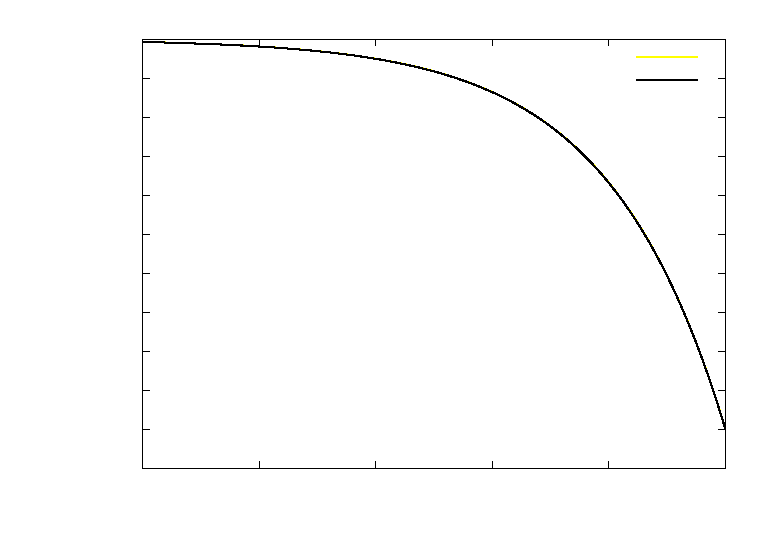
\includegraphics{./Graphics/output_1_neg1_5_1}}%
    \gplfronttext
  \end{picture}%
\endgroup

%% GNUPLOT: LaTeX picture with Postscript
\begingroup
  \makeatletter
  \providecommand\color[2][]{%
    \GenericError{(gnuplot) \space\space\space\@spaces}{%
      Package color not loaded in conjunction with
      terminal option `colourtext'%
    }{See the gnuplot documentation for explanation.%
    }{Either use 'blacktext' in gnuplot or load the package
      color.sty in LaTeX.}%
    \renewcommand\color[2][]{}%
  }%
  \providecommand\includegraphics[2][]{%
    \GenericError{(gnuplot) \space\space\space\@spaces}{%
      Package graphicx or graphics not loaded%
    }{See the gnuplot documentation for explanation.%
    }{The gnuplot epslatex terminal needs graphicx.sty or graphics.sty.}%
    \renewcommand\includegraphics[2][]{}%
  }%
  \providecommand\rotatebox[2]{#2}%
  \@ifundefined{ifGPcolor}{%
    \newif\ifGPcolor
    \GPcolorfalse
  }{}%
  \@ifundefined{ifGPblacktext}{%
    \newif\ifGPblacktext
    \GPblacktexttrue
  }{}%
  % define a \g@addto@macro without @ in the name:
  \let\gplgaddtomacro\g@addto@macro
  % define empty templates for all commands taking text:
  \gdef\gplbacktext{}%
  \gdef\gplfronttext{}%
  \makeatother
  \ifGPblacktext
    % no textcolor at all
    \def\colorrgb#1{}%
    \def\colorgray#1{}%
  \else
    % gray or color?
    \ifGPcolor
      \def\colorrgb#1{\color[rgb]{#1}}%
      \def\colorgray#1{\color[gray]{#1}}%
      \expandafter\def\csname LTw\endcsname{\color{white}}%
      \expandafter\def\csname LTb\endcsname{\color{black}}%
      \expandafter\def\csname LTa\endcsname{\color{black}}%
      \expandafter\def\csname LT0\endcsname{\color[rgb]{1,0,0}}%
      \expandafter\def\csname LT1\endcsname{\color[rgb]{0,1,0}}%
      \expandafter\def\csname LT2\endcsname{\color[rgb]{0,0,1}}%
      \expandafter\def\csname LT3\endcsname{\color[rgb]{1,0,1}}%
      \expandafter\def\csname LT4\endcsname{\color[rgb]{0,1,1}}%
      \expandafter\def\csname LT5\endcsname{\color[rgb]{1,1,0}}%
      \expandafter\def\csname LT6\endcsname{\color[rgb]{0,0,0}}%
      \expandafter\def\csname LT7\endcsname{\color[rgb]{1,0.3,0}}%
      \expandafter\def\csname LT8\endcsname{\color[rgb]{0.5,0.5,0.5}}%
    \else
      % gray
      \def\colorrgb#1{\color{black}}%
      \def\colorgray#1{\color[gray]{#1}}%
      \expandafter\def\csname LTw\endcsname{\color{white}}%
      \expandafter\def\csname LTb\endcsname{\color{black}}%
      \expandafter\def\csname LTa\endcsname{\color{black}}%
      \expandafter\def\csname LT0\endcsname{\color{black}}%
      \expandafter\def\csname LT1\endcsname{\color{black}}%
      \expandafter\def\csname LT2\endcsname{\color{black}}%
      \expandafter\def\csname LT3\endcsname{\color{black}}%
      \expandafter\def\csname LT4\endcsname{\color{black}}%
      \expandafter\def\csname LT5\endcsname{\color{black}}%
      \expandafter\def\csname LT6\endcsname{\color{black}}%
      \expandafter\def\csname LT7\endcsname{\color{black}}%
      \expandafter\def\csname LT8\endcsname{\color{black}}%
    \fi
  \fi
    \setlength{\unitlength}{0.0500bp}%
    \ifx\gptboxheight\undefined%
      \newlength{\gptboxheight}%
      \newlength{\gptboxwidth}%
      \newsavebox{\gptboxtext}%
    \fi%
    \setlength{\fboxrule}{0.5pt}%
    \setlength{\fboxsep}{1pt}%
\begin{picture}(7200.00,5040.00)%
    \gplgaddtomacro\gplbacktext{%
      \csname LTb\endcsname%%
      \put(946,704){\makebox(0,0)[r]{\strut{}$0$}}%
      \put(946,1116){\makebox(0,0)[r]{\strut{}$0.02$}}%
      \put(946,1527){\makebox(0,0)[r]{\strut{}$0.04$}}%
      \put(946,1939){\makebox(0,0)[r]{\strut{}$0.06$}}%
      \put(946,2350){\makebox(0,0)[r]{\strut{}$0.08$}}%
      \put(946,2762){\makebox(0,0)[r]{\strut{}$0.1$}}%
      \put(946,3173){\makebox(0,0)[r]{\strut{}$0.12$}}%
      \put(946,3584){\makebox(0,0)[r]{\strut{}$0.14$}}%
      \put(946,3996){\makebox(0,0)[r]{\strut{}$0.16$}}%
      \put(946,4408){\makebox(0,0)[r]{\strut{}$0.18$}}%
      \put(946,4819){\makebox(0,0)[r]{\strut{}$0.2$}}%
      \put(1078,484){\makebox(0,0){\strut{}$0$}}%
      \put(2223,484){\makebox(0,0){\strut{}$0.2$}}%
      \put(3368,484){\makebox(0,0){\strut{}$0.4$}}%
      \put(4513,484){\makebox(0,0){\strut{}$0.6$}}%
      \put(5658,484){\makebox(0,0){\strut{}$0.8$}}%
      \put(6803,484){\makebox(0,0){\strut{}$1$}}%
    }%
    \gplgaddtomacro\gplfronttext{%
      \csname LTb\endcsname%%
      \put(198,2761){\rotatebox{-270}{\makebox(0,0){\strut{}$Phi(x, mu)$}}}%
      \put(3940,154){\makebox(0,0){\strut{}$x}}%
      \csname LTb\endcsname%%
      \put(5816,4646){\makebox(0,0)[r]{\strut{}théorique}}%
      \csname LTb\endcsname%%
      \put(5816,4426){\makebox(0,0)[r]{\strut{}approximation}}%
    }%
    \gplbacktext
    \put(0,0){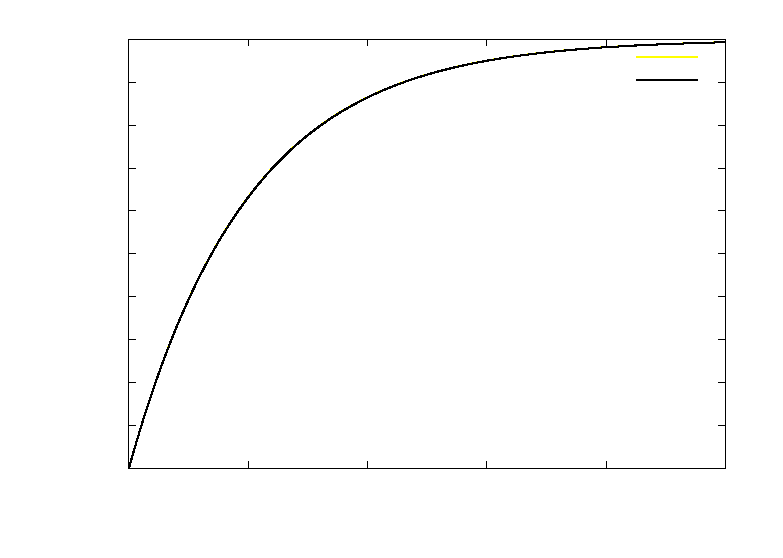
\includegraphics{./output_1_1_5_1}}%
    \gplfronttext
  \end{picture}%
\endgroup

%% GNUPLOT: LaTeX picture with Postscript
\begingroup
  \makeatletter
  \providecommand\color[2][]{%
    \GenericError{(gnuplot) \space\space\space\@spaces}{%
      Package color not loaded in conjunction with
      terminal option `colourtext'%
    }{See the gnuplot documentation for explanation.%
    }{Either use 'blacktext' in gnuplot or load the package
      color.sty in LaTeX.}%
    \renewcommand\color[2][]{}%
  }%
  \providecommand\includegraphics[2][]{%
    \GenericError{(gnuplot) \space\space\space\@spaces}{%
      Package graphicx or graphics not loaded%
    }{See the gnuplot documentation for explanation.%
    }{The gnuplot epslatex terminal needs graphicx.sty or graphics.sty.}%
    \renewcommand\includegraphics[2][]{}%
  }%
  \providecommand\rotatebox[2]{#2}%
  \@ifundefined{ifGPcolor}{%
    \newif\ifGPcolor
    \GPcolorfalse
  }{}%
  \@ifundefined{ifGPblacktext}{%
    \newif\ifGPblacktext
    \GPblacktexttrue
  }{}%
  % define a \g@addto@macro without @ in the name:
  \let\gplgaddtomacro\g@addto@macro
  % define empty templates for all commands taking text:
  \gdef\gplbacktext{}%
  \gdef\gplfronttext{}%
  \makeatother
  \ifGPblacktext
    % no textcolor at all
    \def\colorrgb#1{}%
    \def\colorgray#1{}%
  \else
    % gray or color?
    \ifGPcolor
      \def\colorrgb#1{\color[rgb]{#1}}%
      \def\colorgray#1{\color[gray]{#1}}%
      \expandafter\def\csname LTw\endcsname{\color{white}}%
      \expandafter\def\csname LTb\endcsname{\color{black}}%
      \expandafter\def\csname LTa\endcsname{\color{black}}%
      \expandafter\def\csname LT0\endcsname{\color[rgb]{1,0,0}}%
      \expandafter\def\csname LT1\endcsname{\color[rgb]{0,1,0}}%
      \expandafter\def\csname LT2\endcsname{\color[rgb]{0,0,1}}%
      \expandafter\def\csname LT3\endcsname{\color[rgb]{1,0,1}}%
      \expandafter\def\csname LT4\endcsname{\color[rgb]{0,1,1}}%
      \expandafter\def\csname LT5\endcsname{\color[rgb]{1,1,0}}%
      \expandafter\def\csname LT6\endcsname{\color[rgb]{0,0,0}}%
      \expandafter\def\csname LT7\endcsname{\color[rgb]{1,0.3,0}}%
      \expandafter\def\csname LT8\endcsname{\color[rgb]{0.5,0.5,0.5}}%
    \else
      % gray
      \def\colorrgb#1{\color{black}}%
      \def\colorgray#1{\color[gray]{#1}}%
      \expandafter\def\csname LTw\endcsname{\color{white}}%
      \expandafter\def\csname LTb\endcsname{\color{black}}%
      \expandafter\def\csname LTa\endcsname{\color{black}}%
      \expandafter\def\csname LT0\endcsname{\color{black}}%
      \expandafter\def\csname LT1\endcsname{\color{black}}%
      \expandafter\def\csname LT2\endcsname{\color{black}}%
      \expandafter\def\csname LT3\endcsname{\color{black}}%
      \expandafter\def\csname LT4\endcsname{\color{black}}%
      \expandafter\def\csname LT5\endcsname{\color{black}}%
      \expandafter\def\csname LT6\endcsname{\color{black}}%
      \expandafter\def\csname LT7\endcsname{\color{black}}%
      \expandafter\def\csname LT8\endcsname{\color{black}}%
    \fi
  \fi
    \setlength{\unitlength}{0.0500bp}%
    \ifx\gptboxheight\undefined%
      \newlength{\gptboxheight}%
      \newlength{\gptboxwidth}%
      \newsavebox{\gptboxtext}%
    \fi%
    \setlength{\fboxrule}{0.5pt}%
    \setlength{\fboxsep}{1pt}%
\begin{picture}(7200.00,5040.00)%
    \gplgaddtomacro\gplbacktext{%
      \csname LTb\endcsname%%
      \put(814,704){\makebox(0,0)[r]{\strut{}$0.1$}}%
      \put(814,1161){\makebox(0,0)[r]{\strut{}$0.2$}}%
      \put(814,1618){\makebox(0,0)[r]{\strut{}$0.3$}}%
      \put(814,2076){\makebox(0,0)[r]{\strut{}$0.4$}}%
      \put(814,2533){\makebox(0,0)[r]{\strut{}$0.5$}}%
      \put(814,2990){\makebox(0,0)[r]{\strut{}$0.6$}}%
      \put(814,3447){\makebox(0,0)[r]{\strut{}$0.7$}}%
      \put(814,3905){\makebox(0,0)[r]{\strut{}$0.8$}}%
      \put(814,4362){\makebox(0,0)[r]{\strut{}$0.9$}}%
      \put(814,4819){\makebox(0,0)[r]{\strut{}$1$}}%
      \put(946,484){\makebox(0,0){\strut{}$0$}}%
      \put(2117,484){\makebox(0,0){\strut{}$0.2$}}%
      \put(3289,484){\makebox(0,0){\strut{}$0.4$}}%
      \put(4460,484){\makebox(0,0){\strut{}$0.6$}}%
      \put(5632,484){\makebox(0,0){\strut{}$0.8$}}%
      \put(6803,484){\makebox(0,0){\strut{}$1$}}%
    }%
    \gplgaddtomacro\gplfronttext{%
      \csname LTb\endcsname%%
      \put(198,2761){\rotatebox{-270}{\makebox(0,0){\strut{}$\phi(x, mu)$}}}%
      \put(3874,154){\makebox(0,0){\strut{}$x$}}%
      \csname LTb\endcsname%%
      \put(5816,4646){\makebox(0,0)[r]{\strut{}théorique}}%
      \csname LTb\endcsname%%
      \put(5816,4426){\makebox(0,0)[r]{\strut{}approximation}}%
    }%
    \gplbacktext
    \put(0,0){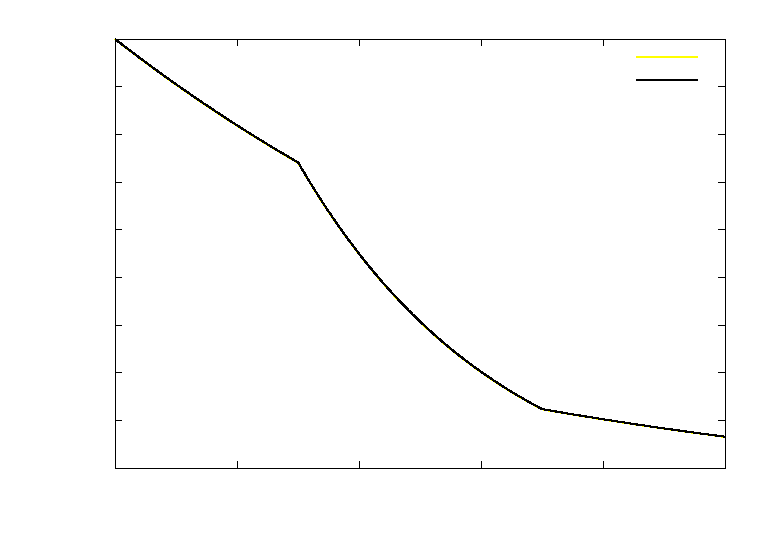
\includegraphics{./Graphics/output_two_steps_1_1_1_2}}%
    \gplfronttext
  \end{picture}%
\endgroup

%% GNUPLOT: LaTeX picture with Postscript
\begingroup
  \makeatletter
  \providecommand\color[2][]{%
    \GenericError{(gnuplot) \space\space\space\@spaces}{%
      Package color not loaded in conjunction with
      terminal option `colourtext'%
    }{See the gnuplot documentation for explanation.%
    }{Either use 'blacktext' in gnuplot or load the package
      color.sty in LaTeX.}%
    \renewcommand\color[2][]{}%
  }%
  \providecommand\includegraphics[2][]{%
    \GenericError{(gnuplot) \space\space\space\@spaces}{%
      Package graphicx or graphics not loaded%
    }{See the gnuplot documentation for explanation.%
    }{The gnuplot epslatex terminal needs graphicx.sty or graphics.sty.}%
    \renewcommand\includegraphics[2][]{}%
  }%
  \providecommand\rotatebox[2]{#2}%
  \@ifundefined{ifGPcolor}{%
    \newif\ifGPcolor
    \GPcolorfalse
  }{}%
  \@ifundefined{ifGPblacktext}{%
    \newif\ifGPblacktext
    \GPblacktexttrue
  }{}%
  % define a \g@addto@macro without @ in the name:
  \let\gplgaddtomacro\g@addto@macro
  % define empty templates for all commands taking text:
  \gdef\gplbacktext{}%
  \gdef\gplfronttext{}%
  \makeatother
  \ifGPblacktext
    % no textcolor at all
    \def\colorrgb#1{}%
    \def\colorgray#1{}%
  \else
    % gray or color?
    \ifGPcolor
      \def\colorrgb#1{\color[rgb]{#1}}%
      \def\colorgray#1{\color[gray]{#1}}%
      \expandafter\def\csname LTw\endcsname{\color{white}}%
      \expandafter\def\csname LTb\endcsname{\color{black}}%
      \expandafter\def\csname LTa\endcsname{\color{black}}%
      \expandafter\def\csname LT0\endcsname{\color[rgb]{1,0,0}}%
      \expandafter\def\csname LT1\endcsname{\color[rgb]{0,1,0}}%
      \expandafter\def\csname LT2\endcsname{\color[rgb]{0,0,1}}%
      \expandafter\def\csname LT3\endcsname{\color[rgb]{1,0,1}}%
      \expandafter\def\csname LT4\endcsname{\color[rgb]{0,1,1}}%
      \expandafter\def\csname LT5\endcsname{\color[rgb]{1,1,0}}%
      \expandafter\def\csname LT6\endcsname{\color[rgb]{0,0,0}}%
      \expandafter\def\csname LT7\endcsname{\color[rgb]{1,0.3,0}}%
      \expandafter\def\csname LT8\endcsname{\color[rgb]{0.5,0.5,0.5}}%
    \else
      % gray
      \def\colorrgb#1{\color{black}}%
      \def\colorgray#1{\color[gray]{#1}}%
      \expandafter\def\csname LTw\endcsname{\color{white}}%
      \expandafter\def\csname LTb\endcsname{\color{black}}%
      \expandafter\def\csname LTa\endcsname{\color{black}}%
      \expandafter\def\csname LT0\endcsname{\color{black}}%
      \expandafter\def\csname LT1\endcsname{\color{black}}%
      \expandafter\def\csname LT2\endcsname{\color{black}}%
      \expandafter\def\csname LT3\endcsname{\color{black}}%
      \expandafter\def\csname LT4\endcsname{\color{black}}%
      \expandafter\def\csname LT5\endcsname{\color{black}}%
      \expandafter\def\csname LT6\endcsname{\color{black}}%
      \expandafter\def\csname LT7\endcsname{\color{black}}%
      \expandafter\def\csname LT8\endcsname{\color{black}}%
    \fi
  \fi
    \setlength{\unitlength}{0.0500bp}%
    \ifx\gptboxheight\undefined%
      \newlength{\gptboxheight}%
      \newlength{\gptboxwidth}%
      \newsavebox{\gptboxtext}%
    \fi%
    \setlength{\fboxrule}{0.5pt}%
    \setlength{\fboxsep}{1pt}%
\begin{picture}(7200.00,5040.00)%
    \gplgaddtomacro\gplbacktext{%
      \csname LTb\endcsname%%
      \put(814,704){\makebox(0,0)[r]{\strut{}$0$}}%
      \put(814,1116){\makebox(0,0)[r]{\strut{}$0.2$}}%
      \put(814,1527){\makebox(0,0)[r]{\strut{}$0.4$}}%
      \put(814,1939){\makebox(0,0)[r]{\strut{}$0.6$}}%
      \put(814,2350){\makebox(0,0)[r]{\strut{}$0.8$}}%
      \put(814,2762){\makebox(0,0)[r]{\strut{}$1$}}%
      \put(814,3173){\makebox(0,0)[r]{\strut{}$1.2$}}%
      \put(814,3585){\makebox(0,0)[r]{\strut{}$1.4$}}%
      \put(814,3996){\makebox(0,0)[r]{\strut{}$1.6$}}%
      \put(814,4408){\makebox(0,0)[r]{\strut{}$1.8$}}%
      \put(814,4819){\makebox(0,0)[r]{\strut{}$2$}}%
      \put(946,484){\makebox(0,0){\strut{}$0$}}%
      \put(2117,484){\makebox(0,0){\strut{}$0.2$}}%
      \put(3289,484){\makebox(0,0){\strut{}$0.4$}}%
      \put(4460,484){\makebox(0,0){\strut{}$0.6$}}%
      \put(5632,484){\makebox(0,0){\strut{}$0.8$}}%
      \put(6803,484){\makebox(0,0){\strut{}$1$}}%
    }%
    \gplgaddtomacro\gplfronttext{%
      \csname LTb\endcsname%%
      \put(198,2761){\rotatebox{-270}{\makebox(0,0){\strut{}$\phi(x, mu)$}}}%
      \put(3874,154){\makebox(0,0){\strut{}$x$}}%
      \csname LTb\endcsname%%
      \put(5816,4646){\makebox(0,0)[r]{\strut{}théorique}}%
      \csname LTb\endcsname%%
      \put(5816,4426){\makebox(0,0)[r]{\strut{}approximation}}%
    }%
    \gplbacktext
    \put(0,0){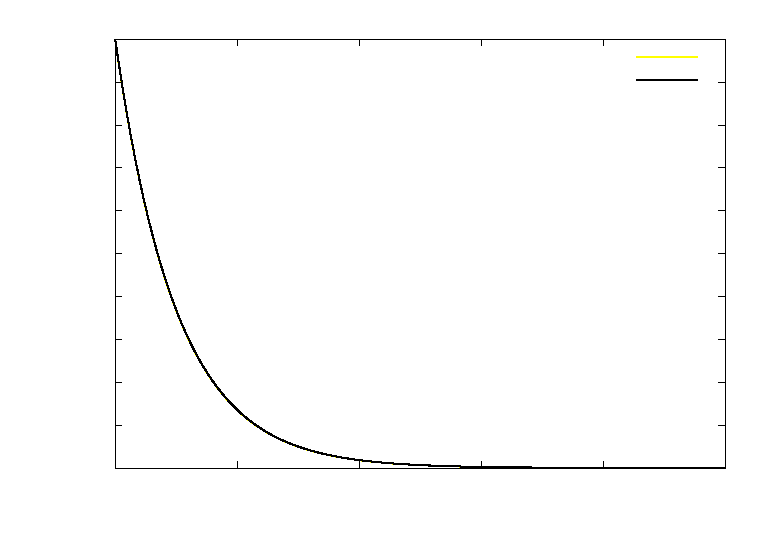
\includegraphics{./Graphics/output_1_05_5_2}}%
    \gplfronttext
  \end{picture}%
\endgroup

%% GNUPLOT: LaTeX picture with Postscript
\begingroup
  \makeatletter
  \providecommand\color[2][]{%
    \GenericError{(gnuplot) \space\space\space\@spaces}{%
      Package color not loaded in conjunction with
      terminal option `colourtext'%
    }{See the gnuplot documentation for explanation.%
    }{Either use 'blacktext' in gnuplot or load the package
      color.sty in LaTeX.}%
    \renewcommand\color[2][]{}%
  }%
  \providecommand\includegraphics[2][]{%
    \GenericError{(gnuplot) \space\space\space\@spaces}{%
      Package graphicx or graphics not loaded%
    }{See the gnuplot documentation for explanation.%
    }{The gnuplot epslatex terminal needs graphicx.sty or graphics.sty.}%
    \renewcommand\includegraphics[2][]{}%
  }%
  \providecommand\rotatebox[2]{#2}%
  \@ifundefined{ifGPcolor}{%
    \newif\ifGPcolor
    \GPcolorfalse
  }{}%
  \@ifundefined{ifGPblacktext}{%
    \newif\ifGPblacktext
    \GPblacktexttrue
  }{}%
  % define a \g@addto@macro without @ in the name:
  \let\gplgaddtomacro\g@addto@macro
  % define empty templates for all commands taking text:
  \gdef\gplbacktext{}%
  \gdef\gplfronttext{}%
  \makeatother
  \ifGPblacktext
    % no textcolor at all
    \def\colorrgb#1{}%
    \def\colorgray#1{}%
  \else
    % gray or color?
    \ifGPcolor
      \def\colorrgb#1{\color[rgb]{#1}}%
      \def\colorgray#1{\color[gray]{#1}}%
      \expandafter\def\csname LTw\endcsname{\color{white}}%
      \expandafter\def\csname LTb\endcsname{\color{black}}%
      \expandafter\def\csname LTa\endcsname{\color{black}}%
      \expandafter\def\csname LT0\endcsname{\color[rgb]{1,0,0}}%
      \expandafter\def\csname LT1\endcsname{\color[rgb]{0,1,0}}%
      \expandafter\def\csname LT2\endcsname{\color[rgb]{0,0,1}}%
      \expandafter\def\csname LT3\endcsname{\color[rgb]{1,0,1}}%
      \expandafter\def\csname LT4\endcsname{\color[rgb]{0,1,1}}%
      \expandafter\def\csname LT5\endcsname{\color[rgb]{1,1,0}}%
      \expandafter\def\csname LT6\endcsname{\color[rgb]{0,0,0}}%
      \expandafter\def\csname LT7\endcsname{\color[rgb]{1,0.3,0}}%
      \expandafter\def\csname LT8\endcsname{\color[rgb]{0.5,0.5,0.5}}%
    \else
      % gray
      \def\colorrgb#1{\color{black}}%
      \def\colorgray#1{\color[gray]{#1}}%
      \expandafter\def\csname LTw\endcsname{\color{white}}%
      \expandafter\def\csname LTb\endcsname{\color{black}}%
      \expandafter\def\csname LTa\endcsname{\color{black}}%
      \expandafter\def\csname LT0\endcsname{\color{black}}%
      \expandafter\def\csname LT1\endcsname{\color{black}}%
      \expandafter\def\csname LT2\endcsname{\color{black}}%
      \expandafter\def\csname LT3\endcsname{\color{black}}%
      \expandafter\def\csname LT4\endcsname{\color{black}}%
      \expandafter\def\csname LT5\endcsname{\color{black}}%
      \expandafter\def\csname LT6\endcsname{\color{black}}%
      \expandafter\def\csname LT7\endcsname{\color{black}}%
      \expandafter\def\csname LT8\endcsname{\color{black}}%
    \fi
  \fi
    \setlength{\unitlength}{0.0500bp}%
    \ifx\gptboxheight\undefined%
      \newlength{\gptboxheight}%
      \newlength{\gptboxwidth}%
      \newsavebox{\gptboxtext}%
    \fi%
    \setlength{\fboxrule}{0.5pt}%
    \setlength{\fboxsep}{1pt}%
\begin{picture}(7200.00,5040.00)%
    \gplgaddtomacro\gplbacktext{%
      \csname LTb\endcsname%%
      \put(814,704){\makebox(0,0)[r]{\strut{}$0$}}%
      \put(814,1116){\makebox(0,0)[r]{\strut{}$0.2$}}%
      \put(814,1527){\makebox(0,0)[r]{\strut{}$0.4$}}%
      \put(814,1939){\makebox(0,0)[r]{\strut{}$0.6$}}%
      \put(814,2350){\makebox(0,0)[r]{\strut{}$0.8$}}%
      \put(814,2762){\makebox(0,0)[r]{\strut{}$1$}}%
      \put(814,3173){\makebox(0,0)[r]{\strut{}$1.2$}}%
      \put(814,3585){\makebox(0,0)[r]{\strut{}$1.4$}}%
      \put(814,3996){\makebox(0,0)[r]{\strut{}$1.6$}}%
      \put(814,4408){\makebox(0,0)[r]{\strut{}$1.8$}}%
      \put(814,4819){\makebox(0,0)[r]{\strut{}$2$}}%
      \put(946,484){\makebox(0,0){\strut{}$0$}}%
      \put(2117,484){\makebox(0,0){\strut{}$0.2$}}%
      \put(3289,484){\makebox(0,0){\strut{}$0.4$}}%
      \put(4460,484){\makebox(0,0){\strut{}$0.6$}}%
      \put(5632,484){\makebox(0,0){\strut{}$0.8$}}%
      \put(6803,484){\makebox(0,0){\strut{}$1$}}%
    }%
    \gplgaddtomacro\gplfronttext{%
      \csname LTb\endcsname%%
      \put(198,2761){\rotatebox{-270}{\makebox(0,0){\strut{}$Phi(x, mu)$}}}%
      \put(3874,154){\makebox(0,0){\strut{}$x}}%
      \csname LTb\endcsname%%
      \put(5816,4646){\makebox(0,0)[r]{\strut{}approximation}}%
    }%
    \gplbacktext
    \put(0,0){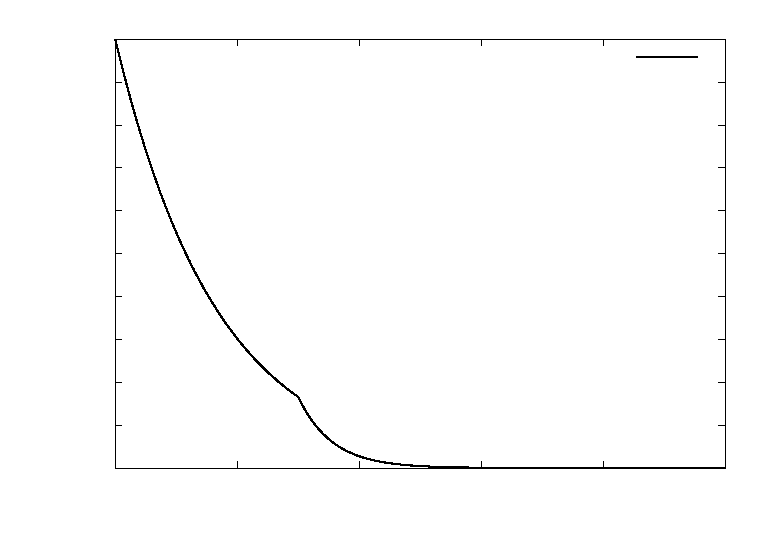
\includegraphics{./Graphics/output_two_steps_1_05_3_2}}%
    \gplfronttext
  \end{picture}%
\endgroup

%% GNUPLOT: LaTeX picture with Postscript
\begingroup
  \makeatletter
  \providecommand\color[2][]{%
    \GenericError{(gnuplot) \space\space\space\@spaces}{%
      Package color not loaded in conjunction with
      terminal option `colourtext'%
    }{See the gnuplot documentation for explanation.%
    }{Either use 'blacktext' in gnuplot or load the package
      color.sty in LaTeX.}%
    \renewcommand\color[2][]{}%
  }%
  \providecommand\includegraphics[2][]{%
    \GenericError{(gnuplot) \space\space\space\@spaces}{%
      Package graphicx or graphics not loaded%
    }{See the gnuplot documentation for explanation.%
    }{The gnuplot epslatex terminal needs graphicx.sty or graphics.sty.}%
    \renewcommand\includegraphics[2][]{}%
  }%
  \providecommand\rotatebox[2]{#2}%
  \@ifundefined{ifGPcolor}{%
    \newif\ifGPcolor
    \GPcolorfalse
  }{}%
  \@ifundefined{ifGPblacktext}{%
    \newif\ifGPblacktext
    \GPblacktexttrue
  }{}%
  % define a \g@addto@macro without @ in the name:
  \let\gplgaddtomacro\g@addto@macro
  % define empty templates for all commands taking text:
  \gdef\gplbacktext{}%
  \gdef\gplfronttext{}%
  \makeatother
  \ifGPblacktext
    % no textcolor at all
    \def\colorrgb#1{}%
    \def\colorgray#1{}%
  \else
    % gray or color?
    \ifGPcolor
      \def\colorrgb#1{\color[rgb]{#1}}%
      \def\colorgray#1{\color[gray]{#1}}%
      \expandafter\def\csname LTw\endcsname{\color{white}}%
      \expandafter\def\csname LTb\endcsname{\color{black}}%
      \expandafter\def\csname LTa\endcsname{\color{black}}%
      \expandafter\def\csname LT0\endcsname{\color[rgb]{1,0,0}}%
      \expandafter\def\csname LT1\endcsname{\color[rgb]{0,1,0}}%
      \expandafter\def\csname LT2\endcsname{\color[rgb]{0,0,1}}%
      \expandafter\def\csname LT3\endcsname{\color[rgb]{1,0,1}}%
      \expandafter\def\csname LT4\endcsname{\color[rgb]{0,1,1}}%
      \expandafter\def\csname LT5\endcsname{\color[rgb]{1,1,0}}%
      \expandafter\def\csname LT6\endcsname{\color[rgb]{0,0,0}}%
      \expandafter\def\csname LT7\endcsname{\color[rgb]{1,0.3,0}}%
      \expandafter\def\csname LT8\endcsname{\color[rgb]{0.5,0.5,0.5}}%
    \else
      % gray
      \def\colorrgb#1{\color{black}}%
      \def\colorgray#1{\color[gray]{#1}}%
      \expandafter\def\csname LTw\endcsname{\color{white}}%
      \expandafter\def\csname LTb\endcsname{\color{black}}%
      \expandafter\def\csname LTa\endcsname{\color{black}}%
      \expandafter\def\csname LT0\endcsname{\color{black}}%
      \expandafter\def\csname LT1\endcsname{\color{black}}%
      \expandafter\def\csname LT2\endcsname{\color{black}}%
      \expandafter\def\csname LT3\endcsname{\color{black}}%
      \expandafter\def\csname LT4\endcsname{\color{black}}%
      \expandafter\def\csname LT5\endcsname{\color{black}}%
      \expandafter\def\csname LT6\endcsname{\color{black}}%
      \expandafter\def\csname LT7\endcsname{\color{black}}%
      \expandafter\def\csname LT8\endcsname{\color{black}}%
    \fi
  \fi
    \setlength{\unitlength}{0.0500bp}%
    \ifx\gptboxheight\undefined%
      \newlength{\gptboxheight}%
      \newlength{\gptboxwidth}%
      \newsavebox{\gptboxtext}%
    \fi%
    \setlength{\fboxrule}{0.5pt}%
    \setlength{\fboxsep}{1pt}%
\begin{picture}(7200.00,5040.00)%
    \gplgaddtomacro\gplbacktext{%
      \csname LTb\endcsname%%
      \put(814,704){\makebox(0,0)[r]{\strut{}$0$}}%
      \put(814,1116){\makebox(0,0)[r]{\strut{}$0.2$}}%
      \put(814,1527){\makebox(0,0)[r]{\strut{}$0.4$}}%
      \put(814,1939){\makebox(0,0)[r]{\strut{}$0.6$}}%
      \put(814,2350){\makebox(0,0)[r]{\strut{}$0.8$}}%
      \put(814,2762){\makebox(0,0)[r]{\strut{}$1$}}%
      \put(814,3173){\makebox(0,0)[r]{\strut{}$1.2$}}%
      \put(814,3585){\makebox(0,0)[r]{\strut{}$1.4$}}%
      \put(814,3996){\makebox(0,0)[r]{\strut{}$1.6$}}%
      \put(814,4408){\makebox(0,0)[r]{\strut{}$1.8$}}%
      \put(814,4819){\makebox(0,0)[r]{\strut{}$2$}}%
      \put(946,484){\makebox(0,0){\strut{}$0$}}%
      \put(2117,484){\makebox(0,0){\strut{}$0.2$}}%
      \put(3289,484){\makebox(0,0){\strut{}$0.4$}}%
      \put(4460,484){\makebox(0,0){\strut{}$0.6$}}%
      \put(5632,484){\makebox(0,0){\strut{}$0.8$}}%
      \put(6803,484){\makebox(0,0){\strut{}$1$}}%
    }%
    \gplgaddtomacro\gplfronttext{%
      \csname LTb\endcsname%%
      \put(198,2761){\rotatebox{-270}{\makebox(0,0){\strut{}$Phi(x, mu)$}}}%
      \put(3874,154){\makebox(0,0){\strut{}$x}}%
      \csname LTb\endcsname%%
      \put(5816,4646){\makebox(0,0)[r]{\strut{}théorique}}%
      \csname LTb\endcsname%%
      \put(5816,4426){\makebox(0,0)[r]{\strut{}approximation}}%
    }%
    \gplbacktext
    \put(0,0){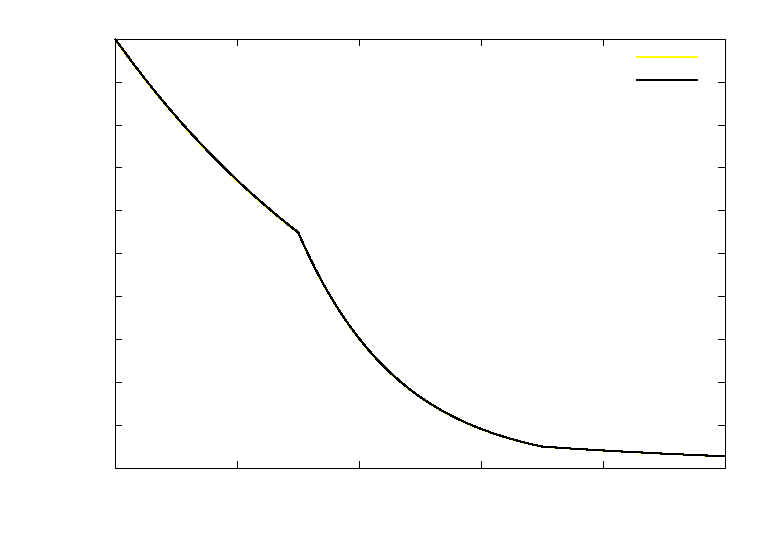
\includegraphics{./Graphics/output_two_steps_1_05_1_2}}%
    \gplfronttext
  \end{picture}%
\endgroup

%% GNUPLOT: LaTeX picture with Postscript
\begingroup
  \makeatletter
  \providecommand\color[2][]{%
    \GenericError{(gnuplot) \space\space\space\@spaces}{%
      Package color not loaded in conjunction with
      terminal option `colourtext'%
    }{See the gnuplot documentation for explanation.%
    }{Either use 'blacktext' in gnuplot or load the package
      color.sty in LaTeX.}%
    \renewcommand\color[2][]{}%
  }%
  \providecommand\includegraphics[2][]{%
    \GenericError{(gnuplot) \space\space\space\@spaces}{%
      Package graphicx or graphics not loaded%
    }{See the gnuplot documentation for explanation.%
    }{The gnuplot epslatex terminal needs graphicx.sty or graphics.sty.}%
    \renewcommand\includegraphics[2][]{}%
  }%
  \providecommand\rotatebox[2]{#2}%
  \@ifundefined{ifGPcolor}{%
    \newif\ifGPcolor
    \GPcolorfalse
  }{}%
  \@ifundefined{ifGPblacktext}{%
    \newif\ifGPblacktext
    \GPblacktexttrue
  }{}%
  % define a \g@addto@macro without @ in the name:
  \let\gplgaddtomacro\g@addto@macro
  % define empty templates for all commands taking text:
  \gdef\gplbacktext{}%
  \gdef\gplfronttext{}%
  \makeatother
  \ifGPblacktext
    % no textcolor at all
    \def\colorrgb#1{}%
    \def\colorgray#1{}%
  \else
    % gray or color?
    \ifGPcolor
      \def\colorrgb#1{\color[rgb]{#1}}%
      \def\colorgray#1{\color[gray]{#1}}%
      \expandafter\def\csname LTw\endcsname{\color{white}}%
      \expandafter\def\csname LTb\endcsname{\color{black}}%
      \expandafter\def\csname LTa\endcsname{\color{black}}%
      \expandafter\def\csname LT0\endcsname{\color[rgb]{1,0,0}}%
      \expandafter\def\csname LT1\endcsname{\color[rgb]{0,1,0}}%
      \expandafter\def\csname LT2\endcsname{\color[rgb]{0,0,1}}%
      \expandafter\def\csname LT3\endcsname{\color[rgb]{1,0,1}}%
      \expandafter\def\csname LT4\endcsname{\color[rgb]{0,1,1}}%
      \expandafter\def\csname LT5\endcsname{\color[rgb]{1,1,0}}%
      \expandafter\def\csname LT6\endcsname{\color[rgb]{0,0,0}}%
      \expandafter\def\csname LT7\endcsname{\color[rgb]{1,0.3,0}}%
      \expandafter\def\csname LT8\endcsname{\color[rgb]{0.5,0.5,0.5}}%
    \else
      % gray
      \def\colorrgb#1{\color{black}}%
      \def\colorgray#1{\color[gray]{#1}}%
      \expandafter\def\csname LTw\endcsname{\color{white}}%
      \expandafter\def\csname LTb\endcsname{\color{black}}%
      \expandafter\def\csname LTa\endcsname{\color{black}}%
      \expandafter\def\csname LT0\endcsname{\color{black}}%
      \expandafter\def\csname LT1\endcsname{\color{black}}%
      \expandafter\def\csname LT2\endcsname{\color{black}}%
      \expandafter\def\csname LT3\endcsname{\color{black}}%
      \expandafter\def\csname LT4\endcsname{\color{black}}%
      \expandafter\def\csname LT5\endcsname{\color{black}}%
      \expandafter\def\csname LT6\endcsname{\color{black}}%
      \expandafter\def\csname LT7\endcsname{\color{black}}%
      \expandafter\def\csname LT8\endcsname{\color{black}}%
    \fi
  \fi
    \setlength{\unitlength}{0.0500bp}%
    \ifx\gptboxheight\undefined%
      \newlength{\gptboxheight}%
      \newlength{\gptboxwidth}%
      \newsavebox{\gptboxtext}%
    \fi%
    \setlength{\fboxrule}{0.5pt}%
    \setlength{\fboxsep}{1pt}%
\begin{picture}(7200.00,5040.00)%
    \gplgaddtomacro\gplbacktext{%
      \csname LTb\endcsname%%
      \put(1078,704){\makebox(0,0)[r]{\strut{}$0$}}%
      \put(1078,1292){\makebox(0,0)[r]{\strut{}$0.005$}}%
      \put(1078,1880){\makebox(0,0)[r]{\strut{}$0.01$}}%
      \put(1078,2468){\makebox(0,0)[r]{\strut{}$0.015$}}%
      \put(1078,3055){\makebox(0,0)[r]{\strut{}$0.02$}}%
      \put(1078,3643){\makebox(0,0)[r]{\strut{}$0.025$}}%
      \put(1078,4231){\makebox(0,0)[r]{\strut{}$0.03$}}%
      \put(1078,4819){\makebox(0,0)[r]{\strut{}$0.035$}}%
      \put(1210,484){\makebox(0,0){\strut{}$0$}}%
      \put(1769,484){\makebox(0,0){\strut{}$100$}}%
      \put(2329,484){\makebox(0,0){\strut{}$200$}}%
      \put(2888,484){\makebox(0,0){\strut{}$300$}}%
      \put(3447,484){\makebox(0,0){\strut{}$400$}}%
      \put(4007,484){\makebox(0,0){\strut{}$500$}}%
      \put(4566,484){\makebox(0,0){\strut{}$600$}}%
      \put(5125,484){\makebox(0,0){\strut{}$700$}}%
      \put(5684,484){\makebox(0,0){\strut{}$800$}}%
      \put(6244,484){\makebox(0,0){\strut{}$900$}}%
      \put(6803,484){\makebox(0,0){\strut{}$1000$}}%
    }%
    \gplgaddtomacro\gplfronttext{%
      \csname LTb\endcsname%%
      \put(198,2761){\rotatebox{-270}{\makebox(0,0){\strut{}Erreur relative $L^2$}}}%
      \put(4006,154){\makebox(0,0){\strut{}$x}}%
      \csname LTb\endcsname%%
      \put(5816,4646){\makebox(0,0)[r]{\strut{}Erreur}}%
    }%
    \gplbacktext
    \put(0,0){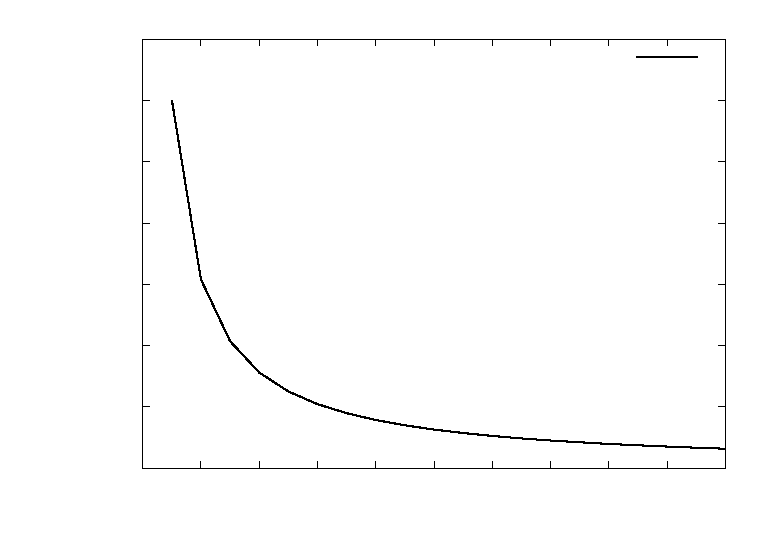
\includegraphics{./Graphics/nb_segs_diff_L2_delta}}%
    \gplfronttext
  \end{picture}%
\endgroup

% GNUPLOT: LaTeX picture with Postscript
\begingroup
  \makeatletter
  \providecommand\color[2][]{%
    \GenericError{(gnuplot) \space\space\space\@spaces}{%
      Package color not loaded in conjunction with
      terminal option `colourtext'%
    }{See the gnuplot documentation for explanation.%
    }{Either use 'blacktext' in gnuplot or load the package
      color.sty in LaTeX.}%
    \renewcommand\color[2][]{}%
  }%
  \providecommand\includegraphics[2][]{%
    \GenericError{(gnuplot) \space\space\space\@spaces}{%
      Package graphicx or graphics not loaded%
    }{See the gnuplot documentation for explanation.%
    }{The gnuplot epslatex terminal needs graphicx.sty or graphics.sty.}%
    \renewcommand\includegraphics[2][]{}%
  }%
  \providecommand\rotatebox[2]{#2}%
  \@ifundefined{ifGPcolor}{%
    \newif\ifGPcolor
    \GPcolorfalse
  }{}%
  \@ifundefined{ifGPblacktext}{%
    \newif\ifGPblacktext
    \GPblacktexttrue
  }{}%
  % define a \g@addto@macro without @ in the name:
  \let\gplgaddtomacro\g@addto@macro
  % define empty templates for all commands taking text:
  \gdef\gplbacktext{}%
  \gdef\gplfronttext{}%
  \makeatother
  \ifGPblacktext
    % no textcolor at all
    \def\colorrgb#1{}%
    \def\colorgray#1{}%
  \else
    % gray or color?
    \ifGPcolor
      \def\colorrgb#1{\color[rgb]{#1}}%
      \def\colorgray#1{\color[gray]{#1}}%
      \expandafter\def\csname LTw\endcsname{\color{white}}%
      \expandafter\def\csname LTb\endcsname{\color{black}}%
      \expandafter\def\csname LTa\endcsname{\color{black}}%
      \expandafter\def\csname LT0\endcsname{\color[rgb]{1,0,0}}%
      \expandafter\def\csname LT1\endcsname{\color[rgb]{0,1,0}}%
      \expandafter\def\csname LT2\endcsname{\color[rgb]{0,0,1}}%
      \expandafter\def\csname LT3\endcsname{\color[rgb]{1,0,1}}%
      \expandafter\def\csname LT4\endcsname{\color[rgb]{0,1,1}}%
      \expandafter\def\csname LT5\endcsname{\color[rgb]{1,1,0}}%
      \expandafter\def\csname LT6\endcsname{\color[rgb]{0,0,0}}%
      \expandafter\def\csname LT7\endcsname{\color[rgb]{1,0.3,0}}%
      \expandafter\def\csname LT8\endcsname{\color[rgb]{0.5,0.5,0.5}}%
    \else
      % gray
      \def\colorrgb#1{\color{black}}%
      \def\colorgray#1{\color[gray]{#1}}%
      \expandafter\def\csname LTw\endcsname{\color{white}}%
      \expandafter\def\csname LTb\endcsname{\color{black}}%
      \expandafter\def\csname LTa\endcsname{\color{black}}%
      \expandafter\def\csname LT0\endcsname{\color{black}}%
      \expandafter\def\csname LT1\endcsname{\color{black}}%
      \expandafter\def\csname LT2\endcsname{\color{black}}%
      \expandafter\def\csname LT3\endcsname{\color{black}}%
      \expandafter\def\csname LT4\endcsname{\color{black}}%
      \expandafter\def\csname LT5\endcsname{\color{black}}%
      \expandafter\def\csname LT6\endcsname{\color{black}}%
      \expandafter\def\csname LT7\endcsname{\color{black}}%
      \expandafter\def\csname LT8\endcsname{\color{black}}%
    \fi
  \fi
    \setlength{\unitlength}{0.0500bp}%
    \ifx\gptboxheight\undefined%
      \newlength{\gptboxheight}%
      \newlength{\gptboxwidth}%
      \newsavebox{\gptboxtext}%
    \fi%
    \setlength{\fboxrule}{0.5pt}%
    \setlength{\fboxsep}{1pt}%
\begin{picture}(7200.00,5040.00)%
    \gplgaddtomacro\gplbacktext{%
      \csname LTb\endcsname%%
      \put(1078,704){\makebox(0,0)[r]{\strut{}$0$}}%
      \put(1078,1390){\makebox(0,0)[r]{\strut{}$0.001$}}%
      \put(1078,2076){\makebox(0,0)[r]{\strut{}$0.002$}}%
      \put(1078,2762){\makebox(0,0)[r]{\strut{}$0.003$}}%
      \put(1078,3447){\makebox(0,0)[r]{\strut{}$0.004$}}%
      \put(1078,4133){\makebox(0,0)[r]{\strut{}$0.005$}}%
      \put(1078,4819){\makebox(0,0)[r]{\strut{}$0.006$}}%
      \put(1210,484){\makebox(0,0){\strut{}$0$}}%
      \put(1769,484){\makebox(0,0){\strut{}$100$}}%
      \put(2329,484){\makebox(0,0){\strut{}$200$}}%
      \put(2888,484){\makebox(0,0){\strut{}$300$}}%
      \put(3447,484){\makebox(0,0){\strut{}$400$}}%
      \put(4007,484){\makebox(0,0){\strut{}$500$}}%
      \put(4566,484){\makebox(0,0){\strut{}$600$}}%
      \put(5125,484){\makebox(0,0){\strut{}$700$}}%
      \put(5684,484){\makebox(0,0){\strut{}$800$}}%
      \put(6244,484){\makebox(0,0){\strut{}$900$}}%
      \put(6803,484){\makebox(0,0){\strut{}$1000$}}%
    }%
    \gplgaddtomacro\gplfronttext{%
      \csname LTb\endcsname%%
      \put(198,2761){\rotatebox{-270}{\makebox(0,0){\strut{}Erreur relative $L^2$}}}%
      \put(4006,154){\makebox(0,0){\strut{}$x}}%
      \csname LTb\endcsname%%
      \put(5816,4646){\makebox(0,0)[r]{\strut{}Erreur}}%
    }%
    \gplbacktext
    \put(0,0){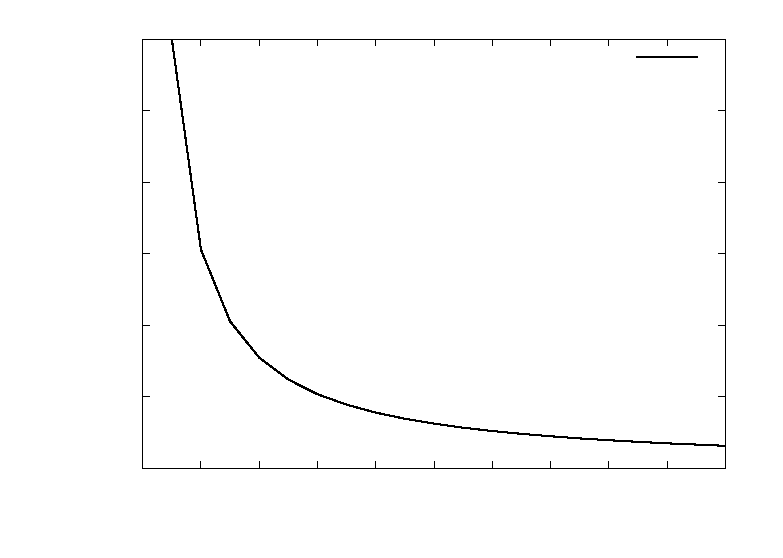
\includegraphics{./Graphics/nb_segs_diff_L2_cste}}%
    \gplfronttext
  \end{picture}%
\endgroup


% GNUPLOT: LaTeX picture with Postscript
\begingroup
  \makeatletter
  \providecommand\color[2][]{%
    \GenericError{(gnuplot) \space\space\space\@spaces}{%
      Package color not loaded in conjunction with
      terminal option `colourtext'%
    }{See the gnuplot documentation for explanation.%
    }{Either use 'blacktext' in gnuplot or load the package
      color.sty in LaTeX.}%
    \renewcommand\color[2][]{}%
  }%
  \providecommand\includegraphics[2][]{%
    \GenericError{(gnuplot) \space\space\space\@spaces}{%
      Package graphicx or graphics not loaded%
    }{See the gnuplot documentation for explanation.%
    }{The gnuplot epslatex terminal needs graphicx.sty or graphics.sty.}%
    \renewcommand\includegraphics[2][]{}%
  }%
  \providecommand\rotatebox[2]{#2}%
  \@ifundefined{ifGPcolor}{%
    \newif\ifGPcolor
    \GPcolorfalse
  }{}%
  \@ifundefined{ifGPblacktext}{%
    \newif\ifGPblacktext
    \GPblacktexttrue
  }{}%
  % define a \g@addto@macro without @ in the name:
  \let\gplgaddtomacro\g@addto@macro
  % define empty templates for all commands taking text:
  \gdef\gplbacktext{}%
  \gdef\gplfronttext{}%
  \makeatother
  \ifGPblacktext
    % no textcolor at all
    \def\colorrgb#1{}%
    \def\colorgray#1{}%
  \else
    % gray or color?
    \ifGPcolor
      \def\colorrgb#1{\color[rgb]{#1}}%
      \def\colorgray#1{\color[gray]{#1}}%
      \expandafter\def\csname LTw\endcsname{\color{white}}%
      \expandafter\def\csname LTb\endcsname{\color{black}}%
      \expandafter\def\csname LTa\endcsname{\color{black}}%
      \expandafter\def\csname LT0\endcsname{\color[rgb]{1,0,0}}%
      \expandafter\def\csname LT1\endcsname{\color[rgb]{0,1,0}}%
      \expandafter\def\csname LT2\endcsname{\color[rgb]{0,0,1}}%
      \expandafter\def\csname LT3\endcsname{\color[rgb]{1,0,1}}%
      \expandafter\def\csname LT4\endcsname{\color[rgb]{0,1,1}}%
      \expandafter\def\csname LT5\endcsname{\color[rgb]{1,1,0}}%
      \expandafter\def\csname LT6\endcsname{\color[rgb]{0,0,0}}%
      \expandafter\def\csname LT7\endcsname{\color[rgb]{1,0.3,0}}%
      \expandafter\def\csname LT8\endcsname{\color[rgb]{0.5,0.5,0.5}}%
    \else
      % gray
      \def\colorrgb#1{\color{black}}%
      \def\colorgray#1{\color[gray]{#1}}%
      \expandafter\def\csname LTw\endcsname{\color{white}}%
      \expandafter\def\csname LTb\endcsname{\color{black}}%
      \expandafter\def\csname LTa\endcsname{\color{black}}%
      \expandafter\def\csname LT0\endcsname{\color{black}}%
      \expandafter\def\csname LT1\endcsname{\color{black}}%
      \expandafter\def\csname LT2\endcsname{\color{black}}%
      \expandafter\def\csname LT3\endcsname{\color{black}}%
      \expandafter\def\csname LT4\endcsname{\color{black}}%
      \expandafter\def\csname LT5\endcsname{\color{black}}%
      \expandafter\def\csname LT6\endcsname{\color{black}}%
      \expandafter\def\csname LT7\endcsname{\color{black}}%
      \expandafter\def\csname LT8\endcsname{\color{black}}%
    \fi
  \fi
    \setlength{\unitlength}{0.0500bp}%
    \ifx\gptboxheight\undefined%
      \newlength{\gptboxheight}%
      \newlength{\gptboxwidth}%
      \newsavebox{\gptboxtext}%
    \fi%
    \setlength{\fboxrule}{0.5pt}%
    \setlength{\fboxsep}{1pt}%
\begin{picture}(7200.00,5040.00)%
    \gplgaddtomacro\gplbacktext{%
      \csname LTb\endcsname%%
      \put(814,704){\makebox(0,0)[r]{\strut{}$0$}}%
      \put(814,1218){\makebox(0,0)[r]{\strut{}$0.5$}}%
      \put(814,1733){\makebox(0,0)[r]{\strut{}$1$}}%
      \put(814,2247){\makebox(0,0)[r]{\strut{}$1.5$}}%
      \put(814,2762){\makebox(0,0)[r]{\strut{}$2$}}%
      \put(814,3276){\makebox(0,0)[r]{\strut{}$2.5$}}%
      \put(814,3790){\makebox(0,0)[r]{\strut{}$3$}}%
      \put(814,4305){\makebox(0,0)[r]{\strut{}$3.5$}}%
      \put(814,4819){\makebox(0,0)[r]{\strut{}$4$}}%
      \put(946,484){\makebox(0,0){\strut{}$0$}}%
      \put(2117,484){\makebox(0,0){\strut{}$0.2$}}%
      \put(3289,484){\makebox(0,0){\strut{}$0.4$}}%
      \put(4460,484){\makebox(0,0){\strut{}$0.6$}}%
      \put(5632,484){\makebox(0,0){\strut{}$0.8$}}%
      \put(6803,484){\makebox(0,0){\strut{}$1$}}%
    }%
    \gplgaddtomacro\gplfronttext{%
      \csname LTb\endcsname%%
      \put(198,2761){\rotatebox{-270}{\makebox(0,0){\strut{}$Phi(x, mu)$}}}%
      \put(3874,154){\makebox(0,0){\strut{}$x}}%
      \csname LTb\endcsname%%
      \put(5816,4646){\makebox(0,0)[r]{\strut{}$N_{\mu}$=2}}%
      \csname LTb\endcsname%%
      \put(5816,4426){\makebox(0,0)[r]{\strut{}$N_{\mu}$=4}}%
      \csname LTb\endcsname%%
      \put(5816,4206){\makebox(0,0)[r]{\strut{}$N_{\mu}$=6}}%
      \csname LTb\endcsname%%
      \put(5816,3986){\makebox(0,0)[r]{\strut{}$N_{\mu}$=8}}%
      \csname LTb\endcsname%%
      \put(5816,3766){\makebox(0,0)[r]{\strut{}$N_{\mu}$=10}}%
      \csname LTb\endcsname%%
      \put(5816,3546){\makebox(0,0)[r]{\strut{}$N_{\mu}$=12}}%
      \csname LTb\endcsname%%
      \put(5816,3326){\makebox(0,0)[r]{\strut{}$N_{\mu}$=14}}%
      \csname LTb\endcsname%%
      \put(5816,3106){\makebox(0,0)[r]{\strut{}$N_{\mu}$=16}}%
    }%
    \gplbacktext
    \put(0,0){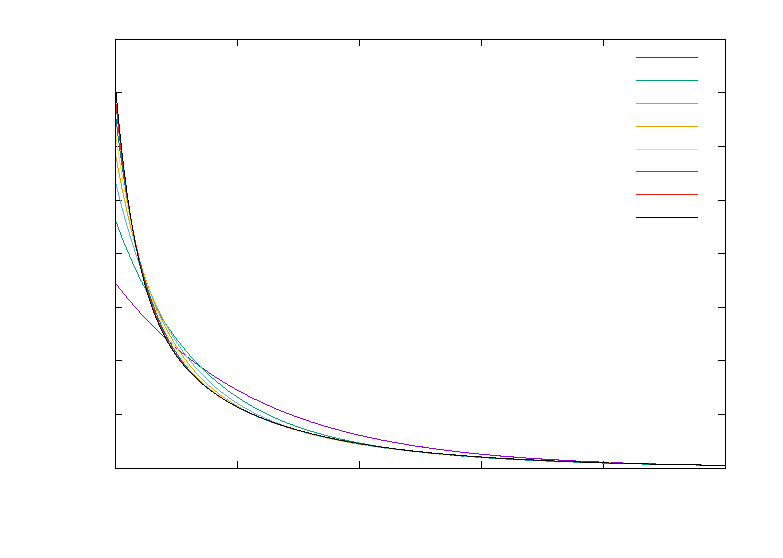
\includegraphics{.\loop_nb_pts_mu_delta.aux}}%
    \gplfronttext
  \end{picture}%
\endgroup

%% GNUPLOT: LaTeX picture with Postscript
\begingroup
  \makeatletter
  \providecommand\color[2][]{%
    \GenericError{(gnuplot) \space\space\space\@spaces}{%
      Package color not loaded in conjunction with
      terminal option `colourtext'%
    }{See the gnuplot documentation for explanation.%
    }{Either use 'blacktext' in gnuplot or load the package
      color.sty in LaTeX.}%
    \renewcommand\color[2][]{}%
  }%
  \providecommand\includegraphics[2][]{%
    \GenericError{(gnuplot) \space\space\space\@spaces}{%
      Package graphicx or graphics not loaded%
    }{See the gnuplot documentation for explanation.%
    }{The gnuplot epslatex terminal needs graphicx.sty or graphics.sty.}%
    \renewcommand\includegraphics[2][]{}%
  }%
  \providecommand\rotatebox[2]{#2}%
  \@ifundefined{ifGPcolor}{%
    \newif\ifGPcolor
    \GPcolorfalse
  }{}%
  \@ifundefined{ifGPblacktext}{%
    \newif\ifGPblacktext
    \GPblacktexttrue
  }{}%
  % define a \g@addto@macro without @ in the name:
  \let\gplgaddtomacro\g@addto@macro
  % define empty templates for all commands taking text:
  \gdef\gplbacktext{}%
  \gdef\gplfronttext{}%
  \makeatother
  \ifGPblacktext
    % no textcolor at all
    \def\colorrgb#1{}%
    \def\colorgray#1{}%
  \else
    % gray or color?
    \ifGPcolor
      \def\colorrgb#1{\color[rgb]{#1}}%
      \def\colorgray#1{\color[gray]{#1}}%
      \expandafter\def\csname LTw\endcsname{\color{white}}%
      \expandafter\def\csname LTb\endcsname{\color{black}}%
      \expandafter\def\csname LTa\endcsname{\color{black}}%
      \expandafter\def\csname LT0\endcsname{\color[rgb]{1,0,0}}%
      \expandafter\def\csname LT1\endcsname{\color[rgb]{0,1,0}}%
      \expandafter\def\csname LT2\endcsname{\color[rgb]{0,0,1}}%
      \expandafter\def\csname LT3\endcsname{\color[rgb]{1,0,1}}%
      \expandafter\def\csname LT4\endcsname{\color[rgb]{0,1,1}}%
      \expandafter\def\csname LT5\endcsname{\color[rgb]{1,1,0}}%
      \expandafter\def\csname LT6\endcsname{\color[rgb]{0,0,0}}%
      \expandafter\def\csname LT7\endcsname{\color[rgb]{1,0.3,0}}%
      \expandafter\def\csname LT8\endcsname{\color[rgb]{0.5,0.5,0.5}}%
    \else
      % gray
      \def\colorrgb#1{\color{black}}%
      \def\colorgray#1{\color[gray]{#1}}%
      \expandafter\def\csname LTw\endcsname{\color{white}}%
      \expandafter\def\csname LTb\endcsname{\color{black}}%
      \expandafter\def\csname LTa\endcsname{\color{black}}%
      \expandafter\def\csname LT0\endcsname{\color{black}}%
      \expandafter\def\csname LT1\endcsname{\color{black}}%
      \expandafter\def\csname LT2\endcsname{\color{black}}%
      \expandafter\def\csname LT3\endcsname{\color{black}}%
      \expandafter\def\csname LT4\endcsname{\color{black}}%
      \expandafter\def\csname LT5\endcsname{\color{black}}%
      \expandafter\def\csname LT6\endcsname{\color{black}}%
      \expandafter\def\csname LT7\endcsname{\color{black}}%
      \expandafter\def\csname LT8\endcsname{\color{black}}%
    \fi
  \fi
    \setlength{\unitlength}{0.0500bp}%
    \ifx\gptboxheight\undefined%
      \newlength{\gptboxheight}%
      \newlength{\gptboxwidth}%
      \newsavebox{\gptboxtext}%
    \fi%
    \setlength{\fboxrule}{0.5pt}%
    \setlength{\fboxsep}{1pt}%
\begin{picture}(7200.00,5040.00)%
    \gplgaddtomacro\gplbacktext{%
      \csname LTb\endcsname%%
      \put(1078,704){\makebox(0,0)[r]{\strut{}$-0.02$}}%
      \put(1078,1078){\makebox(0,0)[r]{\strut{}$0$}}%
      \put(1078,1452){\makebox(0,0)[r]{\strut{}$0.02$}}%
      \put(1078,1826){\makebox(0,0)[r]{\strut{}$0.04$}}%
      \put(1078,2200){\makebox(0,0)[r]{\strut{}$0.06$}}%
      \put(1078,2574){\makebox(0,0)[r]{\strut{}$0.08$}}%
      \put(1078,2949){\makebox(0,0)[r]{\strut{}$0.1$}}%
      \put(1078,3323){\makebox(0,0)[r]{\strut{}$0.12$}}%
      \put(1078,3697){\makebox(0,0)[r]{\strut{}$0.14$}}%
      \put(1078,4071){\makebox(0,0)[r]{\strut{}$0.16$}}%
      \put(1078,4445){\makebox(0,0)[r]{\strut{}$0.18$}}%
      \put(1078,4819){\makebox(0,0)[r]{\strut{}$0.2$}}%
      \put(1210,484){\makebox(0,0){\strut{}$0$}}%
      \put(2329,484){\makebox(0,0){\strut{}$0.2$}}%
      \put(3447,484){\makebox(0,0){\strut{}$0.4$}}%
      \put(4566,484){\makebox(0,0){\strut{}$0.6$}}%
      \put(5684,484){\makebox(0,0){\strut{}$0.8$}}%
      \put(6803,484){\makebox(0,0){\strut{}$1$}}%
    }%
    \gplgaddtomacro\gplfronttext{%
      \csname LTb\endcsname%%
      \put(198,2761){\rotatebox{-270}{\makebox(0,0){\strut{}$\phi(x, mu)$}}}%
      \put(4006,154){\makebox(0,0){\strut{}$x$}}%
      \csname LTb\endcsname%%
      \put(5816,1097){\makebox(0,0)[r]{\strut{}théorique}}%
      \csname LTb\endcsname%%
      \put(5816,877){\makebox(0,0)[r]{\strut{}approximation}}%
    }%
    \gplbacktext
    \put(0,0){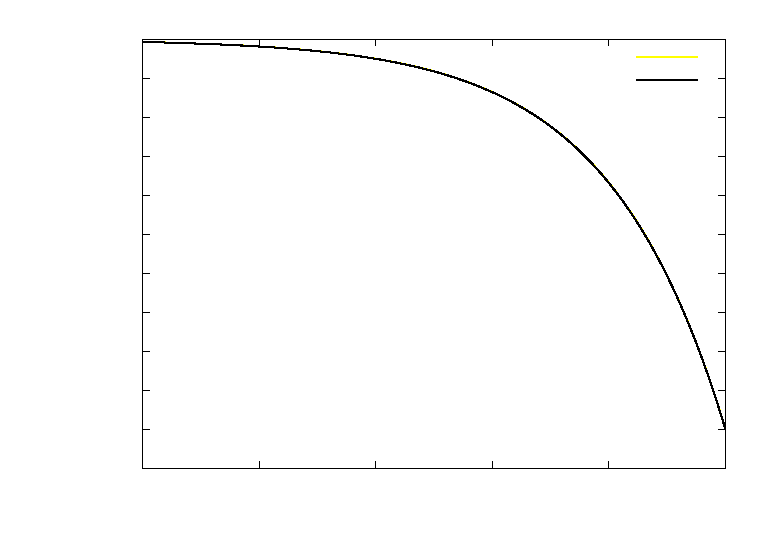
\includegraphics{./Graphics/output_1_neg1_5_1}}%
    \gplfronttext
  \end{picture}%
\endgroup

%% GNUPLOT: LaTeX picture with Postscript
\begingroup
  \makeatletter
  \providecommand\color[2][]{%
    \GenericError{(gnuplot) \space\space\space\@spaces}{%
      Package color not loaded in conjunction with
      terminal option `colourtext'%
    }{See the gnuplot documentation for explanation.%
    }{Either use 'blacktext' in gnuplot or load the package
      color.sty in LaTeX.}%
    \renewcommand\color[2][]{}%
  }%
  \providecommand\includegraphics[2][]{%
    \GenericError{(gnuplot) \space\space\space\@spaces}{%
      Package graphicx or graphics not loaded%
    }{See the gnuplot documentation for explanation.%
    }{The gnuplot epslatex terminal needs graphicx.sty or graphics.sty.}%
    \renewcommand\includegraphics[2][]{}%
  }%
  \providecommand\rotatebox[2]{#2}%
  \@ifundefined{ifGPcolor}{%
    \newif\ifGPcolor
    \GPcolorfalse
  }{}%
  \@ifundefined{ifGPblacktext}{%
    \newif\ifGPblacktext
    \GPblacktexttrue
  }{}%
  % define a \g@addto@macro without @ in the name:
  \let\gplgaddtomacro\g@addto@macro
  % define empty templates for all commands taking text:
  \gdef\gplbacktext{}%
  \gdef\gplfronttext{}%
  \makeatother
  \ifGPblacktext
    % no textcolor at all
    \def\colorrgb#1{}%
    \def\colorgray#1{}%
  \else
    % gray or color?
    \ifGPcolor
      \def\colorrgb#1{\color[rgb]{#1}}%
      \def\colorgray#1{\color[gray]{#1}}%
      \expandafter\def\csname LTw\endcsname{\color{white}}%
      \expandafter\def\csname LTb\endcsname{\color{black}}%
      \expandafter\def\csname LTa\endcsname{\color{black}}%
      \expandafter\def\csname LT0\endcsname{\color[rgb]{1,0,0}}%
      \expandafter\def\csname LT1\endcsname{\color[rgb]{0,1,0}}%
      \expandafter\def\csname LT2\endcsname{\color[rgb]{0,0,1}}%
      \expandafter\def\csname LT3\endcsname{\color[rgb]{1,0,1}}%
      \expandafter\def\csname LT4\endcsname{\color[rgb]{0,1,1}}%
      \expandafter\def\csname LT5\endcsname{\color[rgb]{1,1,0}}%
      \expandafter\def\csname LT6\endcsname{\color[rgb]{0,0,0}}%
      \expandafter\def\csname LT7\endcsname{\color[rgb]{1,0.3,0}}%
      \expandafter\def\csname LT8\endcsname{\color[rgb]{0.5,0.5,0.5}}%
    \else
      % gray
      \def\colorrgb#1{\color{black}}%
      \def\colorgray#1{\color[gray]{#1}}%
      \expandafter\def\csname LTw\endcsname{\color{white}}%
      \expandafter\def\csname LTb\endcsname{\color{black}}%
      \expandafter\def\csname LTa\endcsname{\color{black}}%
      \expandafter\def\csname LT0\endcsname{\color{black}}%
      \expandafter\def\csname LT1\endcsname{\color{black}}%
      \expandafter\def\csname LT2\endcsname{\color{black}}%
      \expandafter\def\csname LT3\endcsname{\color{black}}%
      \expandafter\def\csname LT4\endcsname{\color{black}}%
      \expandafter\def\csname LT5\endcsname{\color{black}}%
      \expandafter\def\csname LT6\endcsname{\color{black}}%
      \expandafter\def\csname LT7\endcsname{\color{black}}%
      \expandafter\def\csname LT8\endcsname{\color{black}}%
    \fi
  \fi
    \setlength{\unitlength}{0.0500bp}%
    \ifx\gptboxheight\undefined%
      \newlength{\gptboxheight}%
      \newlength{\gptboxwidth}%
      \newsavebox{\gptboxtext}%
    \fi%
    \setlength{\fboxrule}{0.5pt}%
    \setlength{\fboxsep}{1pt}%
\begin{picture}(7200.00,5040.00)%
    \gplgaddtomacro\gplbacktext{%
      \csname LTb\endcsname%%
      \put(946,704){\makebox(0,0)[r]{\strut{}$0.4$}}%
      \put(946,1116){\makebox(0,0)[r]{\strut{}$0.45$}}%
      \put(946,1527){\makebox(0,0)[r]{\strut{}$0.5$}}%
      \put(946,1939){\makebox(0,0)[r]{\strut{}$0.55$}}%
      \put(946,2350){\makebox(0,0)[r]{\strut{}$0.6$}}%
      \put(946,2762){\makebox(0,0)[r]{\strut{}$0.65$}}%
      \put(946,3173){\makebox(0,0)[r]{\strut{}$0.7$}}%
      \put(946,3585){\makebox(0,0)[r]{\strut{}$0.75$}}%
      \put(946,3996){\makebox(0,0)[r]{\strut{}$0.8$}}%
      \put(946,4408){\makebox(0,0)[r]{\strut{}$0.85$}}%
      \put(946,4819){\makebox(0,0)[r]{\strut{}$0.9$}}%
      \put(1078,484){\makebox(0,0){\strut{}$0$}}%
      \put(2223,484){\makebox(0,0){\strut{}$0.2$}}%
      \put(3368,484){\makebox(0,0){\strut{}$0.4$}}%
      \put(4513,484){\makebox(0,0){\strut{}$0.6$}}%
      \put(5658,484){\makebox(0,0){\strut{}$0.8$}}%
      \put(6803,484){\makebox(0,0){\strut{}$1$}}%
    }%
    \gplgaddtomacro\gplfronttext{%
      \csname LTb\endcsname%%
      \put(198,2761){\rotatebox{-270}{\makebox(0,0){\strut{}$Phi(x, mu)$}}}%
      \put(3940,154){\makebox(0,0){\strut{}$x}}%
      \csname LTb\endcsname%%
      \put(5816,4646){\makebox(0,0)[r]{\strut{}$N_{\mu}$=2}}%
      \csname LTb\endcsname%%
      \put(5816,4426){\makebox(0,0)[r]{\strut{}$N_{\mu}$=4}}%
      \csname LTb\endcsname%%
      \put(5816,4206){\makebox(0,0)[r]{\strut{}$N_{\mu}$=6}}%
      \csname LTb\endcsname%%
      \put(5816,3986){\makebox(0,0)[r]{\strut{}$N_{\mu}$=8}}%
      \csname LTb\endcsname%%
      \put(5816,3766){\makebox(0,0)[r]{\strut{}$N_{\mu}$=10}}%
      \csname LTb\endcsname%%
      \put(5816,3546){\makebox(0,0)[r]{\strut{}$N_{\mu}$=12}}%
      \csname LTb\endcsname%%
      \put(5816,3326){\makebox(0,0)[r]{\strut{}$N_{\mu}$=14}}%
      \csname LTb\endcsname%%
      \put(5816,3106){\makebox(0,0)[r]{\strut{}$N_{\mu}$=16}}%
    }%
    \gplbacktext
    \put(0,0){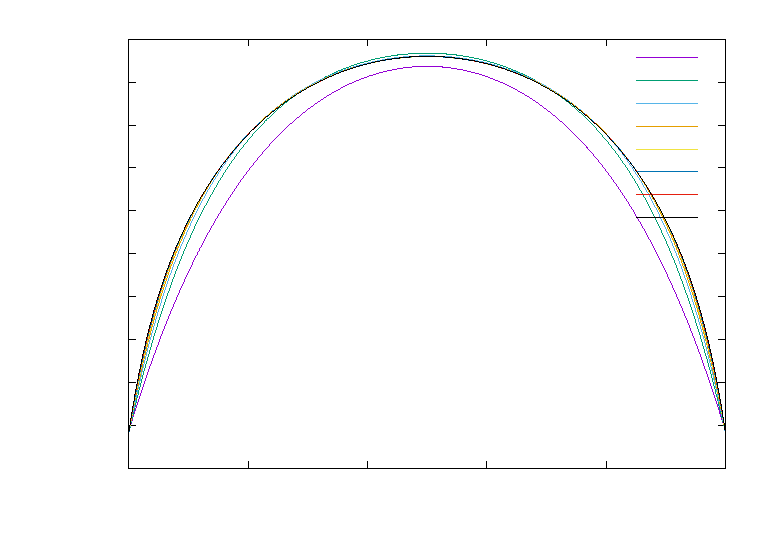
\includegraphics{.\loop_nb_pts_mu_cste}}%
    \gplfronttext
  \end{picture}%
\endgroup

%% GNUPLOT: LaTeX picture with Postscript
\begingroup
  \makeatletter
  \providecommand\color[2][]{%
    \GenericError{(gnuplot) \space\space\space\@spaces}{%
      Package color not loaded in conjunction with
      terminal option `colourtext'%
    }{See the gnuplot documentation for explanation.%
    }{Either use 'blacktext' in gnuplot or load the package
      color.sty in LaTeX.}%
    \renewcommand\color[2][]{}%
  }%
  \providecommand\includegraphics[2][]{%
    \GenericError{(gnuplot) \space\space\space\@spaces}{%
      Package graphicx or graphics not loaded%
    }{See the gnuplot documentation for explanation.%
    }{The gnuplot epslatex terminal needs graphicx.sty or graphics.sty.}%
    \renewcommand\includegraphics[2][]{}%
  }%
  \providecommand\rotatebox[2]{#2}%
  \@ifundefined{ifGPcolor}{%
    \newif\ifGPcolor
    \GPcolorfalse
  }{}%
  \@ifundefined{ifGPblacktext}{%
    \newif\ifGPblacktext
    \GPblacktexttrue
  }{}%
  % define a \g@addto@macro without @ in the name:
  \let\gplgaddtomacro\g@addto@macro
  % define empty templates for all commands taking text:
  \gdef\gplbacktext{}%
  \gdef\gplfronttext{}%
  \makeatother
  \ifGPblacktext
    % no textcolor at all
    \def\colorrgb#1{}%
    \def\colorgray#1{}%
  \else
    % gray or color?
    \ifGPcolor
      \def\colorrgb#1{\color[rgb]{#1}}%
      \def\colorgray#1{\color[gray]{#1}}%
      \expandafter\def\csname LTw\endcsname{\color{white}}%
      \expandafter\def\csname LTb\endcsname{\color{black}}%
      \expandafter\def\csname LTa\endcsname{\color{black}}%
      \expandafter\def\csname LT0\endcsname{\color[rgb]{1,0,0}}%
      \expandafter\def\csname LT1\endcsname{\color[rgb]{0,1,0}}%
      \expandafter\def\csname LT2\endcsname{\color[rgb]{0,0,1}}%
      \expandafter\def\csname LT3\endcsname{\color[rgb]{1,0,1}}%
      \expandafter\def\csname LT4\endcsname{\color[rgb]{0,1,1}}%
      \expandafter\def\csname LT5\endcsname{\color[rgb]{1,1,0}}%
      \expandafter\def\csname LT6\endcsname{\color[rgb]{0,0,0}}%
      \expandafter\def\csname LT7\endcsname{\color[rgb]{1,0.3,0}}%
      \expandafter\def\csname LT8\endcsname{\color[rgb]{0.5,0.5,0.5}}%
    \else
      % gray
      \def\colorrgb#1{\color{black}}%
      \def\colorgray#1{\color[gray]{#1}}%
      \expandafter\def\csname LTw\endcsname{\color{white}}%
      \expandafter\def\csname LTb\endcsname{\color{black}}%
      \expandafter\def\csname LTa\endcsname{\color{black}}%
      \expandafter\def\csname LT0\endcsname{\color{black}}%
      \expandafter\def\csname LT1\endcsname{\color{black}}%
      \expandafter\def\csname LT2\endcsname{\color{black}}%
      \expandafter\def\csname LT3\endcsname{\color{black}}%
      \expandafter\def\csname LT4\endcsname{\color{black}}%
      \expandafter\def\csname LT5\endcsname{\color{black}}%
      \expandafter\def\csname LT6\endcsname{\color{black}}%
      \expandafter\def\csname LT7\endcsname{\color{black}}%
      \expandafter\def\csname LT8\endcsname{\color{black}}%
    \fi
  \fi
    \setlength{\unitlength}{0.0500bp}%
    \ifx\gptboxheight\undefined%
      \newlength{\gptboxheight}%
      \newlength{\gptboxwidth}%
      \newsavebox{\gptboxtext}%
    \fi%
    \setlength{\fboxrule}{0.5pt}%
    \setlength{\fboxsep}{1pt}%
\begin{picture}(7200.00,5040.00)%
    \gplgaddtomacro\gplbacktext{%
      \csname LTb\endcsname%%
      \put(946,704){\makebox(0,0)[r]{\strut{}$0$}}%
      \put(946,1116){\makebox(0,0)[r]{\strut{}$0.02$}}%
      \put(946,1527){\makebox(0,0)[r]{\strut{}$0.04$}}%
      \put(946,1939){\makebox(0,0)[r]{\strut{}$0.06$}}%
      \put(946,2350){\makebox(0,0)[r]{\strut{}$0.08$}}%
      \put(946,2762){\makebox(0,0)[r]{\strut{}$0.1$}}%
      \put(946,3173){\makebox(0,0)[r]{\strut{}$0.12$}}%
      \put(946,3584){\makebox(0,0)[r]{\strut{}$0.14$}}%
      \put(946,3996){\makebox(0,0)[r]{\strut{}$0.16$}}%
      \put(946,4408){\makebox(0,0)[r]{\strut{}$0.18$}}%
      \put(946,4819){\makebox(0,0)[r]{\strut{}$0.2$}}%
      \put(1078,484){\makebox(0,0){\strut{}$0$}}%
      \put(2223,484){\makebox(0,0){\strut{}$0.2$}}%
      \put(3368,484){\makebox(0,0){\strut{}$0.4$}}%
      \put(4513,484){\makebox(0,0){\strut{}$0.6$}}%
      \put(5658,484){\makebox(0,0){\strut{}$0.8$}}%
      \put(6803,484){\makebox(0,0){\strut{}$1$}}%
    }%
    \gplgaddtomacro\gplfronttext{%
      \csname LTb\endcsname%%
      \put(198,2761){\rotatebox{-270}{\makebox(0,0){\strut{}$Phi(x, mu)$}}}%
      \put(3940,154){\makebox(0,0){\strut{}$x}}%
      \csname LTb\endcsname%%
      \put(5816,4646){\makebox(0,0)[r]{\strut{}théorique}}%
      \csname LTb\endcsname%%
      \put(5816,4426){\makebox(0,0)[r]{\strut{}approximation}}%
    }%
    \gplbacktext
    \put(0,0){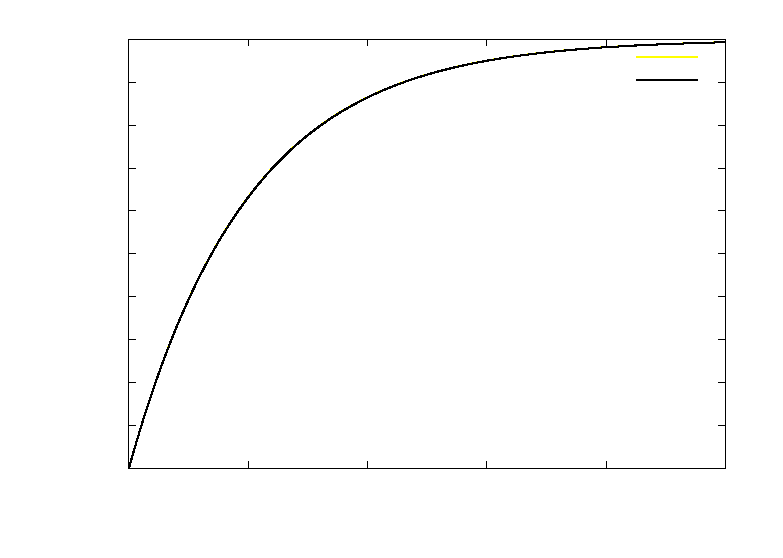
\includegraphics{./output_1_1_5_1}}%
    \gplfronttext
  \end{picture}%
\endgroup

%% GNUPLOT: LaTeX picture with Postscript
\begingroup
  \makeatletter
  \providecommand\color[2][]{%
    \GenericError{(gnuplot) \space\space\space\@spaces}{%
      Package color not loaded in conjunction with
      terminal option `colourtext'%
    }{See the gnuplot documentation for explanation.%
    }{Either use 'blacktext' in gnuplot or load the package
      color.sty in LaTeX.}%
    \renewcommand\color[2][]{}%
  }%
  \providecommand\includegraphics[2][]{%
    \GenericError{(gnuplot) \space\space\space\@spaces}{%
      Package graphicx or graphics not loaded%
    }{See the gnuplot documentation for explanation.%
    }{The gnuplot epslatex terminal needs graphicx.sty or graphics.sty.}%
    \renewcommand\includegraphics[2][]{}%
  }%
  \providecommand\rotatebox[2]{#2}%
  \@ifundefined{ifGPcolor}{%
    \newif\ifGPcolor
    \GPcolorfalse
  }{}%
  \@ifundefined{ifGPblacktext}{%
    \newif\ifGPblacktext
    \GPblacktexttrue
  }{}%
  % define a \g@addto@macro without @ in the name:
  \let\gplgaddtomacro\g@addto@macro
  % define empty templates for all commands taking text:
  \gdef\gplbacktext{}%
  \gdef\gplfronttext{}%
  \makeatother
  \ifGPblacktext
    % no textcolor at all
    \def\colorrgb#1{}%
    \def\colorgray#1{}%
  \else
    % gray or color?
    \ifGPcolor
      \def\colorrgb#1{\color[rgb]{#1}}%
      \def\colorgray#1{\color[gray]{#1}}%
      \expandafter\def\csname LTw\endcsname{\color{white}}%
      \expandafter\def\csname LTb\endcsname{\color{black}}%
      \expandafter\def\csname LTa\endcsname{\color{black}}%
      \expandafter\def\csname LT0\endcsname{\color[rgb]{1,0,0}}%
      \expandafter\def\csname LT1\endcsname{\color[rgb]{0,1,0}}%
      \expandafter\def\csname LT2\endcsname{\color[rgb]{0,0,1}}%
      \expandafter\def\csname LT3\endcsname{\color[rgb]{1,0,1}}%
      \expandafter\def\csname LT4\endcsname{\color[rgb]{0,1,1}}%
      \expandafter\def\csname LT5\endcsname{\color[rgb]{1,1,0}}%
      \expandafter\def\csname LT6\endcsname{\color[rgb]{0,0,0}}%
      \expandafter\def\csname LT7\endcsname{\color[rgb]{1,0.3,0}}%
      \expandafter\def\csname LT8\endcsname{\color[rgb]{0.5,0.5,0.5}}%
    \else
      % gray
      \def\colorrgb#1{\color{black}}%
      \def\colorgray#1{\color[gray]{#1}}%
      \expandafter\def\csname LTw\endcsname{\color{white}}%
      \expandafter\def\csname LTb\endcsname{\color{black}}%
      \expandafter\def\csname LTa\endcsname{\color{black}}%
      \expandafter\def\csname LT0\endcsname{\color{black}}%
      \expandafter\def\csname LT1\endcsname{\color{black}}%
      \expandafter\def\csname LT2\endcsname{\color{black}}%
      \expandafter\def\csname LT3\endcsname{\color{black}}%
      \expandafter\def\csname LT4\endcsname{\color{black}}%
      \expandafter\def\csname LT5\endcsname{\color{black}}%
      \expandafter\def\csname LT6\endcsname{\color{black}}%
      \expandafter\def\csname LT7\endcsname{\color{black}}%
      \expandafter\def\csname LT8\endcsname{\color{black}}%
    \fi
  \fi
    \setlength{\unitlength}{0.0500bp}%
    \ifx\gptboxheight\undefined%
      \newlength{\gptboxheight}%
      \newlength{\gptboxwidth}%
      \newsavebox{\gptboxtext}%
    \fi%
    \setlength{\fboxrule}{0.5pt}%
    \setlength{\fboxsep}{1pt}%
\begin{picture}(7200.00,5040.00)%
    \gplgaddtomacro\gplbacktext{%
      \csname LTb\endcsname%%
      \put(814,704){\makebox(0,0)[r]{\strut{}$0.1$}}%
      \put(814,1161){\makebox(0,0)[r]{\strut{}$0.2$}}%
      \put(814,1618){\makebox(0,0)[r]{\strut{}$0.3$}}%
      \put(814,2076){\makebox(0,0)[r]{\strut{}$0.4$}}%
      \put(814,2533){\makebox(0,0)[r]{\strut{}$0.5$}}%
      \put(814,2990){\makebox(0,0)[r]{\strut{}$0.6$}}%
      \put(814,3447){\makebox(0,0)[r]{\strut{}$0.7$}}%
      \put(814,3905){\makebox(0,0)[r]{\strut{}$0.8$}}%
      \put(814,4362){\makebox(0,0)[r]{\strut{}$0.9$}}%
      \put(814,4819){\makebox(0,0)[r]{\strut{}$1$}}%
      \put(946,484){\makebox(0,0){\strut{}$0$}}%
      \put(2117,484){\makebox(0,0){\strut{}$0.2$}}%
      \put(3289,484){\makebox(0,0){\strut{}$0.4$}}%
      \put(4460,484){\makebox(0,0){\strut{}$0.6$}}%
      \put(5632,484){\makebox(0,0){\strut{}$0.8$}}%
      \put(6803,484){\makebox(0,0){\strut{}$1$}}%
    }%
    \gplgaddtomacro\gplfronttext{%
      \csname LTb\endcsname%%
      \put(198,2761){\rotatebox{-270}{\makebox(0,0){\strut{}$\phi(x, mu)$}}}%
      \put(3874,154){\makebox(0,0){\strut{}$x$}}%
      \csname LTb\endcsname%%
      \put(5816,4646){\makebox(0,0)[r]{\strut{}théorique}}%
      \csname LTb\endcsname%%
      \put(5816,4426){\makebox(0,0)[r]{\strut{}approximation}}%
    }%
    \gplbacktext
    \put(0,0){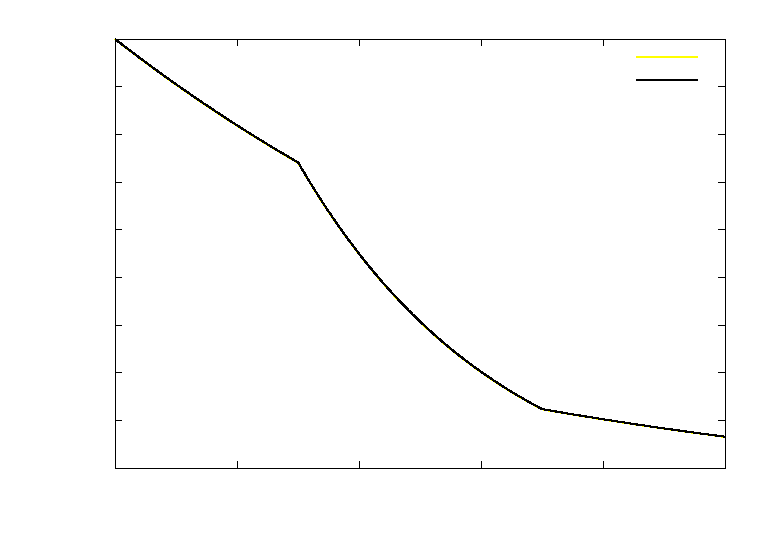
\includegraphics{./Graphics/output_two_steps_1_1_1_2}}%
    \gplfronttext
  \end{picture}%
\endgroup

%% GNUPLOT: LaTeX picture with Postscript
\begingroup
  \makeatletter
  \providecommand\color[2][]{%
    \GenericError{(gnuplot) \space\space\space\@spaces}{%
      Package color not loaded in conjunction with
      terminal option `colourtext'%
    }{See the gnuplot documentation for explanation.%
    }{Either use 'blacktext' in gnuplot or load the package
      color.sty in LaTeX.}%
    \renewcommand\color[2][]{}%
  }%
  \providecommand\includegraphics[2][]{%
    \GenericError{(gnuplot) \space\space\space\@spaces}{%
      Package graphicx or graphics not loaded%
    }{See the gnuplot documentation for explanation.%
    }{The gnuplot epslatex terminal needs graphicx.sty or graphics.sty.}%
    \renewcommand\includegraphics[2][]{}%
  }%
  \providecommand\rotatebox[2]{#2}%
  \@ifundefined{ifGPcolor}{%
    \newif\ifGPcolor
    \GPcolorfalse
  }{}%
  \@ifundefined{ifGPblacktext}{%
    \newif\ifGPblacktext
    \GPblacktexttrue
  }{}%
  % define a \g@addto@macro without @ in the name:
  \let\gplgaddtomacro\g@addto@macro
  % define empty templates for all commands taking text:
  \gdef\gplbacktext{}%
  \gdef\gplfronttext{}%
  \makeatother
  \ifGPblacktext
    % no textcolor at all
    \def\colorrgb#1{}%
    \def\colorgray#1{}%
  \else
    % gray or color?
    \ifGPcolor
      \def\colorrgb#1{\color[rgb]{#1}}%
      \def\colorgray#1{\color[gray]{#1}}%
      \expandafter\def\csname LTw\endcsname{\color{white}}%
      \expandafter\def\csname LTb\endcsname{\color{black}}%
      \expandafter\def\csname LTa\endcsname{\color{black}}%
      \expandafter\def\csname LT0\endcsname{\color[rgb]{1,0,0}}%
      \expandafter\def\csname LT1\endcsname{\color[rgb]{0,1,0}}%
      \expandafter\def\csname LT2\endcsname{\color[rgb]{0,0,1}}%
      \expandafter\def\csname LT3\endcsname{\color[rgb]{1,0,1}}%
      \expandafter\def\csname LT4\endcsname{\color[rgb]{0,1,1}}%
      \expandafter\def\csname LT5\endcsname{\color[rgb]{1,1,0}}%
      \expandafter\def\csname LT6\endcsname{\color[rgb]{0,0,0}}%
      \expandafter\def\csname LT7\endcsname{\color[rgb]{1,0.3,0}}%
      \expandafter\def\csname LT8\endcsname{\color[rgb]{0.5,0.5,0.5}}%
    \else
      % gray
      \def\colorrgb#1{\color{black}}%
      \def\colorgray#1{\color[gray]{#1}}%
      \expandafter\def\csname LTw\endcsname{\color{white}}%
      \expandafter\def\csname LTb\endcsname{\color{black}}%
      \expandafter\def\csname LTa\endcsname{\color{black}}%
      \expandafter\def\csname LT0\endcsname{\color{black}}%
      \expandafter\def\csname LT1\endcsname{\color{black}}%
      \expandafter\def\csname LT2\endcsname{\color{black}}%
      \expandafter\def\csname LT3\endcsname{\color{black}}%
      \expandafter\def\csname LT4\endcsname{\color{black}}%
      \expandafter\def\csname LT5\endcsname{\color{black}}%
      \expandafter\def\csname LT6\endcsname{\color{black}}%
      \expandafter\def\csname LT7\endcsname{\color{black}}%
      \expandafter\def\csname LT8\endcsname{\color{black}}%
    \fi
  \fi
    \setlength{\unitlength}{0.0500bp}%
    \ifx\gptboxheight\undefined%
      \newlength{\gptboxheight}%
      \newlength{\gptboxwidth}%
      \newsavebox{\gptboxtext}%
    \fi%
    \setlength{\fboxrule}{0.5pt}%
    \setlength{\fboxsep}{1pt}%
\begin{picture}(7200.00,5040.00)%
    \gplgaddtomacro\gplbacktext{%
      \csname LTb\endcsname%%
      \put(814,704){\makebox(0,0)[r]{\strut{}$0$}}%
      \put(814,1116){\makebox(0,0)[r]{\strut{}$0.2$}}%
      \put(814,1527){\makebox(0,0)[r]{\strut{}$0.4$}}%
      \put(814,1939){\makebox(0,0)[r]{\strut{}$0.6$}}%
      \put(814,2350){\makebox(0,0)[r]{\strut{}$0.8$}}%
      \put(814,2762){\makebox(0,0)[r]{\strut{}$1$}}%
      \put(814,3173){\makebox(0,0)[r]{\strut{}$1.2$}}%
      \put(814,3585){\makebox(0,0)[r]{\strut{}$1.4$}}%
      \put(814,3996){\makebox(0,0)[r]{\strut{}$1.6$}}%
      \put(814,4408){\makebox(0,0)[r]{\strut{}$1.8$}}%
      \put(814,4819){\makebox(0,0)[r]{\strut{}$2$}}%
      \put(946,484){\makebox(0,0){\strut{}$0$}}%
      \put(2117,484){\makebox(0,0){\strut{}$0.2$}}%
      \put(3289,484){\makebox(0,0){\strut{}$0.4$}}%
      \put(4460,484){\makebox(0,0){\strut{}$0.6$}}%
      \put(5632,484){\makebox(0,0){\strut{}$0.8$}}%
      \put(6803,484){\makebox(0,0){\strut{}$1$}}%
    }%
    \gplgaddtomacro\gplfronttext{%
      \csname LTb\endcsname%%
      \put(198,2761){\rotatebox{-270}{\makebox(0,0){\strut{}$\phi(x, mu)$}}}%
      \put(3874,154){\makebox(0,0){\strut{}$x$}}%
      \csname LTb\endcsname%%
      \put(5816,4646){\makebox(0,0)[r]{\strut{}théorique}}%
      \csname LTb\endcsname%%
      \put(5816,4426){\makebox(0,0)[r]{\strut{}approximation}}%
    }%
    \gplbacktext
    \put(0,0){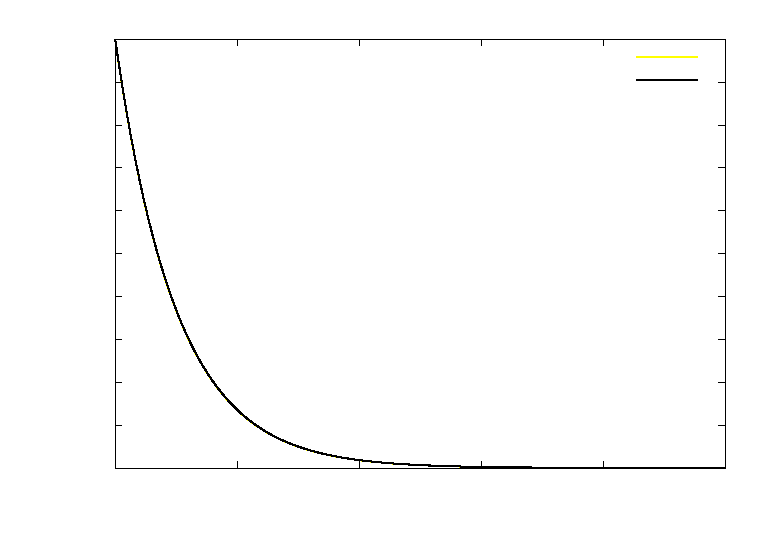
\includegraphics{./Graphics/output_1_05_5_2}}%
    \gplfronttext
  \end{picture}%
\endgroup

%% GNUPLOT: LaTeX picture with Postscript
\begingroup
  \makeatletter
  \providecommand\color[2][]{%
    \GenericError{(gnuplot) \space\space\space\@spaces}{%
      Package color not loaded in conjunction with
      terminal option `colourtext'%
    }{See the gnuplot documentation for explanation.%
    }{Either use 'blacktext' in gnuplot or load the package
      color.sty in LaTeX.}%
    \renewcommand\color[2][]{}%
  }%
  \providecommand\includegraphics[2][]{%
    \GenericError{(gnuplot) \space\space\space\@spaces}{%
      Package graphicx or graphics not loaded%
    }{See the gnuplot documentation for explanation.%
    }{The gnuplot epslatex terminal needs graphicx.sty or graphics.sty.}%
    \renewcommand\includegraphics[2][]{}%
  }%
  \providecommand\rotatebox[2]{#2}%
  \@ifundefined{ifGPcolor}{%
    \newif\ifGPcolor
    \GPcolorfalse
  }{}%
  \@ifundefined{ifGPblacktext}{%
    \newif\ifGPblacktext
    \GPblacktexttrue
  }{}%
  % define a \g@addto@macro without @ in the name:
  \let\gplgaddtomacro\g@addto@macro
  % define empty templates for all commands taking text:
  \gdef\gplbacktext{}%
  \gdef\gplfronttext{}%
  \makeatother
  \ifGPblacktext
    % no textcolor at all
    \def\colorrgb#1{}%
    \def\colorgray#1{}%
  \else
    % gray or color?
    \ifGPcolor
      \def\colorrgb#1{\color[rgb]{#1}}%
      \def\colorgray#1{\color[gray]{#1}}%
      \expandafter\def\csname LTw\endcsname{\color{white}}%
      \expandafter\def\csname LTb\endcsname{\color{black}}%
      \expandafter\def\csname LTa\endcsname{\color{black}}%
      \expandafter\def\csname LT0\endcsname{\color[rgb]{1,0,0}}%
      \expandafter\def\csname LT1\endcsname{\color[rgb]{0,1,0}}%
      \expandafter\def\csname LT2\endcsname{\color[rgb]{0,0,1}}%
      \expandafter\def\csname LT3\endcsname{\color[rgb]{1,0,1}}%
      \expandafter\def\csname LT4\endcsname{\color[rgb]{0,1,1}}%
      \expandafter\def\csname LT5\endcsname{\color[rgb]{1,1,0}}%
      \expandafter\def\csname LT6\endcsname{\color[rgb]{0,0,0}}%
      \expandafter\def\csname LT7\endcsname{\color[rgb]{1,0.3,0}}%
      \expandafter\def\csname LT8\endcsname{\color[rgb]{0.5,0.5,0.5}}%
    \else
      % gray
      \def\colorrgb#1{\color{black}}%
      \def\colorgray#1{\color[gray]{#1}}%
      \expandafter\def\csname LTw\endcsname{\color{white}}%
      \expandafter\def\csname LTb\endcsname{\color{black}}%
      \expandafter\def\csname LTa\endcsname{\color{black}}%
      \expandafter\def\csname LT0\endcsname{\color{black}}%
      \expandafter\def\csname LT1\endcsname{\color{black}}%
      \expandafter\def\csname LT2\endcsname{\color{black}}%
      \expandafter\def\csname LT3\endcsname{\color{black}}%
      \expandafter\def\csname LT4\endcsname{\color{black}}%
      \expandafter\def\csname LT5\endcsname{\color{black}}%
      \expandafter\def\csname LT6\endcsname{\color{black}}%
      \expandafter\def\csname LT7\endcsname{\color{black}}%
      \expandafter\def\csname LT8\endcsname{\color{black}}%
    \fi
  \fi
    \setlength{\unitlength}{0.0500bp}%
    \ifx\gptboxheight\undefined%
      \newlength{\gptboxheight}%
      \newlength{\gptboxwidth}%
      \newsavebox{\gptboxtext}%
    \fi%
    \setlength{\fboxrule}{0.5pt}%
    \setlength{\fboxsep}{1pt}%
\begin{picture}(7200.00,5040.00)%
    \gplgaddtomacro\gplbacktext{%
      \csname LTb\endcsname%%
      \put(814,704){\makebox(0,0)[r]{\strut{}$0$}}%
      \put(814,1116){\makebox(0,0)[r]{\strut{}$0.2$}}%
      \put(814,1527){\makebox(0,0)[r]{\strut{}$0.4$}}%
      \put(814,1939){\makebox(0,0)[r]{\strut{}$0.6$}}%
      \put(814,2350){\makebox(0,0)[r]{\strut{}$0.8$}}%
      \put(814,2762){\makebox(0,0)[r]{\strut{}$1$}}%
      \put(814,3173){\makebox(0,0)[r]{\strut{}$1.2$}}%
      \put(814,3585){\makebox(0,0)[r]{\strut{}$1.4$}}%
      \put(814,3996){\makebox(0,0)[r]{\strut{}$1.6$}}%
      \put(814,4408){\makebox(0,0)[r]{\strut{}$1.8$}}%
      \put(814,4819){\makebox(0,0)[r]{\strut{}$2$}}%
      \put(946,484){\makebox(0,0){\strut{}$0$}}%
      \put(2117,484){\makebox(0,0){\strut{}$0.2$}}%
      \put(3289,484){\makebox(0,0){\strut{}$0.4$}}%
      \put(4460,484){\makebox(0,0){\strut{}$0.6$}}%
      \put(5632,484){\makebox(0,0){\strut{}$0.8$}}%
      \put(6803,484){\makebox(0,0){\strut{}$1$}}%
    }%
    \gplgaddtomacro\gplfronttext{%
      \csname LTb\endcsname%%
      \put(198,2761){\rotatebox{-270}{\makebox(0,0){\strut{}$Phi(x, mu)$}}}%
      \put(3874,154){\makebox(0,0){\strut{}$x}}%
      \csname LTb\endcsname%%
      \put(5816,4646){\makebox(0,0)[r]{\strut{}approximation}}%
    }%
    \gplbacktext
    \put(0,0){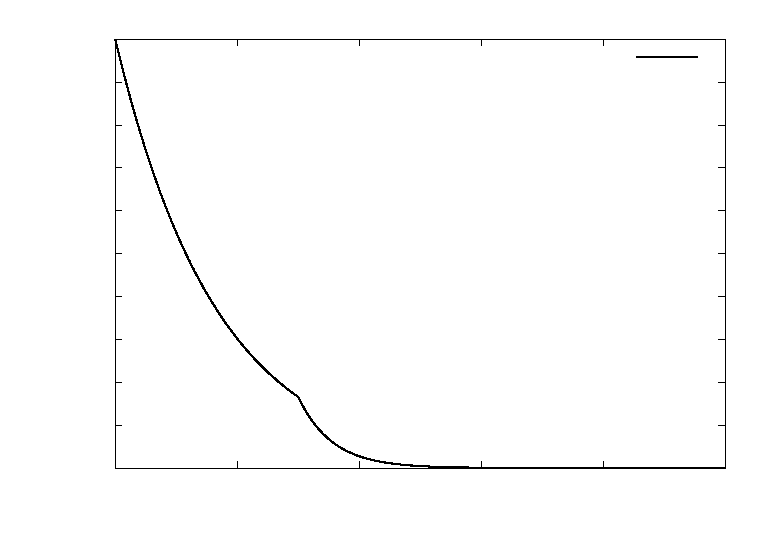
\includegraphics{./Graphics/output_two_steps_1_05_3_2}}%
    \gplfronttext
  \end{picture}%
\endgroup

%% GNUPLOT: LaTeX picture with Postscript
\begingroup
  \makeatletter
  \providecommand\color[2][]{%
    \GenericError{(gnuplot) \space\space\space\@spaces}{%
      Package color not loaded in conjunction with
      terminal option `colourtext'%
    }{See the gnuplot documentation for explanation.%
    }{Either use 'blacktext' in gnuplot or load the package
      color.sty in LaTeX.}%
    \renewcommand\color[2][]{}%
  }%
  \providecommand\includegraphics[2][]{%
    \GenericError{(gnuplot) \space\space\space\@spaces}{%
      Package graphicx or graphics not loaded%
    }{See the gnuplot documentation for explanation.%
    }{The gnuplot epslatex terminal needs graphicx.sty or graphics.sty.}%
    \renewcommand\includegraphics[2][]{}%
  }%
  \providecommand\rotatebox[2]{#2}%
  \@ifundefined{ifGPcolor}{%
    \newif\ifGPcolor
    \GPcolorfalse
  }{}%
  \@ifundefined{ifGPblacktext}{%
    \newif\ifGPblacktext
    \GPblacktexttrue
  }{}%
  % define a \g@addto@macro without @ in the name:
  \let\gplgaddtomacro\g@addto@macro
  % define empty templates for all commands taking text:
  \gdef\gplbacktext{}%
  \gdef\gplfronttext{}%
  \makeatother
  \ifGPblacktext
    % no textcolor at all
    \def\colorrgb#1{}%
    \def\colorgray#1{}%
  \else
    % gray or color?
    \ifGPcolor
      \def\colorrgb#1{\color[rgb]{#1}}%
      \def\colorgray#1{\color[gray]{#1}}%
      \expandafter\def\csname LTw\endcsname{\color{white}}%
      \expandafter\def\csname LTb\endcsname{\color{black}}%
      \expandafter\def\csname LTa\endcsname{\color{black}}%
      \expandafter\def\csname LT0\endcsname{\color[rgb]{1,0,0}}%
      \expandafter\def\csname LT1\endcsname{\color[rgb]{0,1,0}}%
      \expandafter\def\csname LT2\endcsname{\color[rgb]{0,0,1}}%
      \expandafter\def\csname LT3\endcsname{\color[rgb]{1,0,1}}%
      \expandafter\def\csname LT4\endcsname{\color[rgb]{0,1,1}}%
      \expandafter\def\csname LT5\endcsname{\color[rgb]{1,1,0}}%
      \expandafter\def\csname LT6\endcsname{\color[rgb]{0,0,0}}%
      \expandafter\def\csname LT7\endcsname{\color[rgb]{1,0.3,0}}%
      \expandafter\def\csname LT8\endcsname{\color[rgb]{0.5,0.5,0.5}}%
    \else
      % gray
      \def\colorrgb#1{\color{black}}%
      \def\colorgray#1{\color[gray]{#1}}%
      \expandafter\def\csname LTw\endcsname{\color{white}}%
      \expandafter\def\csname LTb\endcsname{\color{black}}%
      \expandafter\def\csname LTa\endcsname{\color{black}}%
      \expandafter\def\csname LT0\endcsname{\color{black}}%
      \expandafter\def\csname LT1\endcsname{\color{black}}%
      \expandafter\def\csname LT2\endcsname{\color{black}}%
      \expandafter\def\csname LT3\endcsname{\color{black}}%
      \expandafter\def\csname LT4\endcsname{\color{black}}%
      \expandafter\def\csname LT5\endcsname{\color{black}}%
      \expandafter\def\csname LT6\endcsname{\color{black}}%
      \expandafter\def\csname LT7\endcsname{\color{black}}%
      \expandafter\def\csname LT8\endcsname{\color{black}}%
    \fi
  \fi
    \setlength{\unitlength}{0.0500bp}%
    \ifx\gptboxheight\undefined%
      \newlength{\gptboxheight}%
      \newlength{\gptboxwidth}%
      \newsavebox{\gptboxtext}%
    \fi%
    \setlength{\fboxrule}{0.5pt}%
    \setlength{\fboxsep}{1pt}%
\begin{picture}(7200.00,5040.00)%
    \gplgaddtomacro\gplbacktext{%
      \csname LTb\endcsname%%
      \put(814,704){\makebox(0,0)[r]{\strut{}$0$}}%
      \put(814,1116){\makebox(0,0)[r]{\strut{}$0.2$}}%
      \put(814,1527){\makebox(0,0)[r]{\strut{}$0.4$}}%
      \put(814,1939){\makebox(0,0)[r]{\strut{}$0.6$}}%
      \put(814,2350){\makebox(0,0)[r]{\strut{}$0.8$}}%
      \put(814,2762){\makebox(0,0)[r]{\strut{}$1$}}%
      \put(814,3173){\makebox(0,0)[r]{\strut{}$1.2$}}%
      \put(814,3585){\makebox(0,0)[r]{\strut{}$1.4$}}%
      \put(814,3996){\makebox(0,0)[r]{\strut{}$1.6$}}%
      \put(814,4408){\makebox(0,0)[r]{\strut{}$1.8$}}%
      \put(814,4819){\makebox(0,0)[r]{\strut{}$2$}}%
      \put(946,484){\makebox(0,0){\strut{}$0$}}%
      \put(2117,484){\makebox(0,0){\strut{}$0.2$}}%
      \put(3289,484){\makebox(0,0){\strut{}$0.4$}}%
      \put(4460,484){\makebox(0,0){\strut{}$0.6$}}%
      \put(5632,484){\makebox(0,0){\strut{}$0.8$}}%
      \put(6803,484){\makebox(0,0){\strut{}$1$}}%
    }%
    \gplgaddtomacro\gplfronttext{%
      \csname LTb\endcsname%%
      \put(198,2761){\rotatebox{-270}{\makebox(0,0){\strut{}$Phi(x, mu)$}}}%
      \put(3874,154){\makebox(0,0){\strut{}$x}}%
      \csname LTb\endcsname%%
      \put(5816,4646){\makebox(0,0)[r]{\strut{}théorique}}%
      \csname LTb\endcsname%%
      \put(5816,4426){\makebox(0,0)[r]{\strut{}approximation}}%
    }%
    \gplbacktext
    \put(0,0){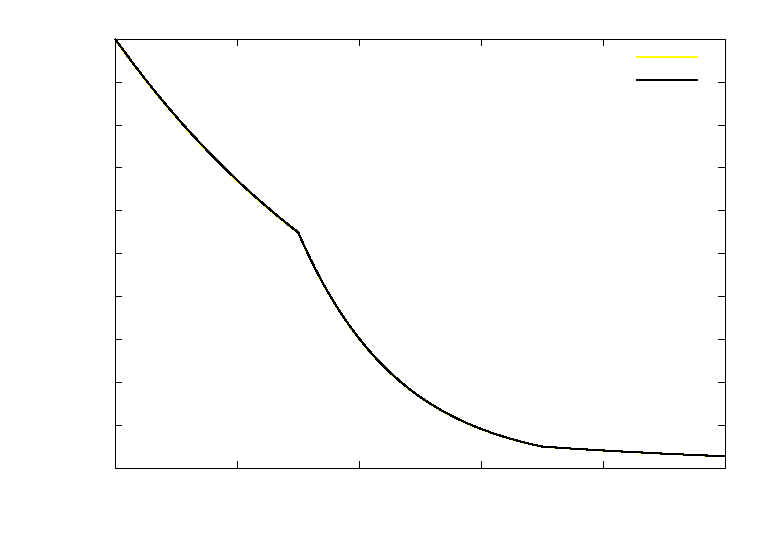
\includegraphics{./Graphics/output_two_steps_1_05_1_2}}%
    \gplfronttext
  \end{picture}%
\endgroup

%% GNUPLOT: LaTeX picture with Postscript
\begingroup
  \makeatletter
  \providecommand\color[2][]{%
    \GenericError{(gnuplot) \space\space\space\@spaces}{%
      Package color not loaded in conjunction with
      terminal option `colourtext'%
    }{See the gnuplot documentation for explanation.%
    }{Either use 'blacktext' in gnuplot or load the package
      color.sty in LaTeX.}%
    \renewcommand\color[2][]{}%
  }%
  \providecommand\includegraphics[2][]{%
    \GenericError{(gnuplot) \space\space\space\@spaces}{%
      Package graphicx or graphics not loaded%
    }{See the gnuplot documentation for explanation.%
    }{The gnuplot epslatex terminal needs graphicx.sty or graphics.sty.}%
    \renewcommand\includegraphics[2][]{}%
  }%
  \providecommand\rotatebox[2]{#2}%
  \@ifundefined{ifGPcolor}{%
    \newif\ifGPcolor
    \GPcolorfalse
  }{}%
  \@ifundefined{ifGPblacktext}{%
    \newif\ifGPblacktext
    \GPblacktexttrue
  }{}%
  % define a \g@addto@macro without @ in the name:
  \let\gplgaddtomacro\g@addto@macro
  % define empty templates for all commands taking text:
  \gdef\gplbacktext{}%
  \gdef\gplfronttext{}%
  \makeatother
  \ifGPblacktext
    % no textcolor at all
    \def\colorrgb#1{}%
    \def\colorgray#1{}%
  \else
    % gray or color?
    \ifGPcolor
      \def\colorrgb#1{\color[rgb]{#1}}%
      \def\colorgray#1{\color[gray]{#1}}%
      \expandafter\def\csname LTw\endcsname{\color{white}}%
      \expandafter\def\csname LTb\endcsname{\color{black}}%
      \expandafter\def\csname LTa\endcsname{\color{black}}%
      \expandafter\def\csname LT0\endcsname{\color[rgb]{1,0,0}}%
      \expandafter\def\csname LT1\endcsname{\color[rgb]{0,1,0}}%
      \expandafter\def\csname LT2\endcsname{\color[rgb]{0,0,1}}%
      \expandafter\def\csname LT3\endcsname{\color[rgb]{1,0,1}}%
      \expandafter\def\csname LT4\endcsname{\color[rgb]{0,1,1}}%
      \expandafter\def\csname LT5\endcsname{\color[rgb]{1,1,0}}%
      \expandafter\def\csname LT6\endcsname{\color[rgb]{0,0,0}}%
      \expandafter\def\csname LT7\endcsname{\color[rgb]{1,0.3,0}}%
      \expandafter\def\csname LT8\endcsname{\color[rgb]{0.5,0.5,0.5}}%
    \else
      % gray
      \def\colorrgb#1{\color{black}}%
      \def\colorgray#1{\color[gray]{#1}}%
      \expandafter\def\csname LTw\endcsname{\color{white}}%
      \expandafter\def\csname LTb\endcsname{\color{black}}%
      \expandafter\def\csname LTa\endcsname{\color{black}}%
      \expandafter\def\csname LT0\endcsname{\color{black}}%
      \expandafter\def\csname LT1\endcsname{\color{black}}%
      \expandafter\def\csname LT2\endcsname{\color{black}}%
      \expandafter\def\csname LT3\endcsname{\color{black}}%
      \expandafter\def\csname LT4\endcsname{\color{black}}%
      \expandafter\def\csname LT5\endcsname{\color{black}}%
      \expandafter\def\csname LT6\endcsname{\color{black}}%
      \expandafter\def\csname LT7\endcsname{\color{black}}%
      \expandafter\def\csname LT8\endcsname{\color{black}}%
    \fi
  \fi
    \setlength{\unitlength}{0.0500bp}%
    \ifx\gptboxheight\undefined%
      \newlength{\gptboxheight}%
      \newlength{\gptboxwidth}%
      \newsavebox{\gptboxtext}%
    \fi%
    \setlength{\fboxrule}{0.5pt}%
    \setlength{\fboxsep}{1pt}%
\begin{picture}(7200.00,5040.00)%
    \gplgaddtomacro\gplbacktext{%
      \csname LTb\endcsname%%
      \put(1078,704){\makebox(0,0)[r]{\strut{}$0$}}%
      \put(1078,1292){\makebox(0,0)[r]{\strut{}$0.005$}}%
      \put(1078,1880){\makebox(0,0)[r]{\strut{}$0.01$}}%
      \put(1078,2468){\makebox(0,0)[r]{\strut{}$0.015$}}%
      \put(1078,3055){\makebox(0,0)[r]{\strut{}$0.02$}}%
      \put(1078,3643){\makebox(0,0)[r]{\strut{}$0.025$}}%
      \put(1078,4231){\makebox(0,0)[r]{\strut{}$0.03$}}%
      \put(1078,4819){\makebox(0,0)[r]{\strut{}$0.035$}}%
      \put(1210,484){\makebox(0,0){\strut{}$0$}}%
      \put(1769,484){\makebox(0,0){\strut{}$100$}}%
      \put(2329,484){\makebox(0,0){\strut{}$200$}}%
      \put(2888,484){\makebox(0,0){\strut{}$300$}}%
      \put(3447,484){\makebox(0,0){\strut{}$400$}}%
      \put(4007,484){\makebox(0,0){\strut{}$500$}}%
      \put(4566,484){\makebox(0,0){\strut{}$600$}}%
      \put(5125,484){\makebox(0,0){\strut{}$700$}}%
      \put(5684,484){\makebox(0,0){\strut{}$800$}}%
      \put(6244,484){\makebox(0,0){\strut{}$900$}}%
      \put(6803,484){\makebox(0,0){\strut{}$1000$}}%
    }%
    \gplgaddtomacro\gplfronttext{%
      \csname LTb\endcsname%%
      \put(198,2761){\rotatebox{-270}{\makebox(0,0){\strut{}Erreur relative $L^2$}}}%
      \put(4006,154){\makebox(0,0){\strut{}$x}}%
      \csname LTb\endcsname%%
      \put(5816,4646){\makebox(0,0)[r]{\strut{}Erreur}}%
    }%
    \gplbacktext
    \put(0,0){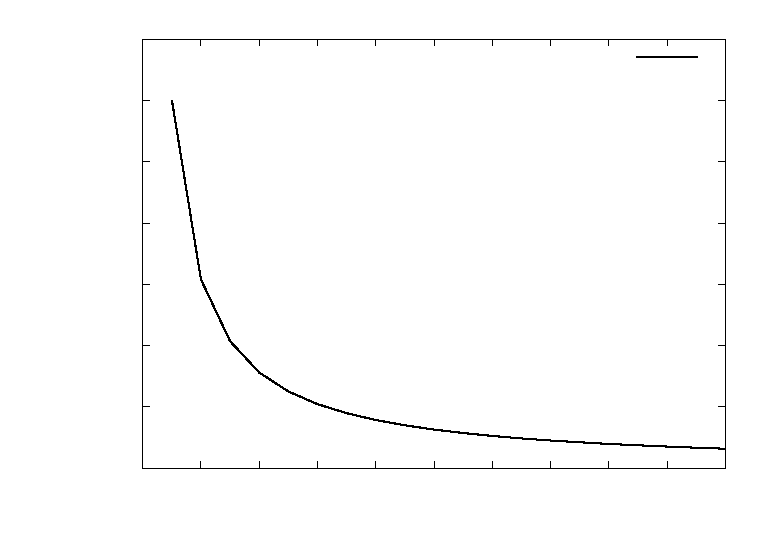
\includegraphics{./Graphics/nb_segs_diff_L2_delta}}%
    \gplfronttext
  \end{picture}%
\endgroup

%% GNUPLOT: LaTeX picture with Postscript
\begingroup
  \makeatletter
  \providecommand\color[2][]{%
    \GenericError{(gnuplot) \space\space\space\@spaces}{%
      Package color not loaded in conjunction with
      terminal option `colourtext'%
    }{See the gnuplot documentation for explanation.%
    }{Either use 'blacktext' in gnuplot or load the package
      color.sty in LaTeX.}%
    \renewcommand\color[2][]{}%
  }%
  \providecommand\includegraphics[2][]{%
    \GenericError{(gnuplot) \space\space\space\@spaces}{%
      Package graphicx or graphics not loaded%
    }{See the gnuplot documentation for explanation.%
    }{The gnuplot epslatex terminal needs graphicx.sty or graphics.sty.}%
    \renewcommand\includegraphics[2][]{}%
  }%
  \providecommand\rotatebox[2]{#2}%
  \@ifundefined{ifGPcolor}{%
    \newif\ifGPcolor
    \GPcolorfalse
  }{}%
  \@ifundefined{ifGPblacktext}{%
    \newif\ifGPblacktext
    \GPblacktexttrue
  }{}%
  % define a \g@addto@macro without @ in the name:
  \let\gplgaddtomacro\g@addto@macro
  % define empty templates for all commands taking text:
  \gdef\gplbacktext{}%
  \gdef\gplfronttext{}%
  \makeatother
  \ifGPblacktext
    % no textcolor at all
    \def\colorrgb#1{}%
    \def\colorgray#1{}%
  \else
    % gray or color?
    \ifGPcolor
      \def\colorrgb#1{\color[rgb]{#1}}%
      \def\colorgray#1{\color[gray]{#1}}%
      \expandafter\def\csname LTw\endcsname{\color{white}}%
      \expandafter\def\csname LTb\endcsname{\color{black}}%
      \expandafter\def\csname LTa\endcsname{\color{black}}%
      \expandafter\def\csname LT0\endcsname{\color[rgb]{1,0,0}}%
      \expandafter\def\csname LT1\endcsname{\color[rgb]{0,1,0}}%
      \expandafter\def\csname LT2\endcsname{\color[rgb]{0,0,1}}%
      \expandafter\def\csname LT3\endcsname{\color[rgb]{1,0,1}}%
      \expandafter\def\csname LT4\endcsname{\color[rgb]{0,1,1}}%
      \expandafter\def\csname LT5\endcsname{\color[rgb]{1,1,0}}%
      \expandafter\def\csname LT6\endcsname{\color[rgb]{0,0,0}}%
      \expandafter\def\csname LT7\endcsname{\color[rgb]{1,0.3,0}}%
      \expandafter\def\csname LT8\endcsname{\color[rgb]{0.5,0.5,0.5}}%
    \else
      % gray
      \def\colorrgb#1{\color{black}}%
      \def\colorgray#1{\color[gray]{#1}}%
      \expandafter\def\csname LTw\endcsname{\color{white}}%
      \expandafter\def\csname LTb\endcsname{\color{black}}%
      \expandafter\def\csname LTa\endcsname{\color{black}}%
      \expandafter\def\csname LT0\endcsname{\color{black}}%
      \expandafter\def\csname LT1\endcsname{\color{black}}%
      \expandafter\def\csname LT2\endcsname{\color{black}}%
      \expandafter\def\csname LT3\endcsname{\color{black}}%
      \expandafter\def\csname LT4\endcsname{\color{black}}%
      \expandafter\def\csname LT5\endcsname{\color{black}}%
      \expandafter\def\csname LT6\endcsname{\color{black}}%
      \expandafter\def\csname LT7\endcsname{\color{black}}%
      \expandafter\def\csname LT8\endcsname{\color{black}}%
    \fi
  \fi
    \setlength{\unitlength}{0.0500bp}%
    \ifx\gptboxheight\undefined%
      \newlength{\gptboxheight}%
      \newlength{\gptboxwidth}%
      \newsavebox{\gptboxtext}%
    \fi%
    \setlength{\fboxrule}{0.5pt}%
    \setlength{\fboxsep}{1pt}%
\begin{picture}(7200.00,5040.00)%
    \gplgaddtomacro\gplbacktext{%
      \csname LTb\endcsname%%
      \put(1078,704){\makebox(0,0)[r]{\strut{}$0$}}%
      \put(1078,1390){\makebox(0,0)[r]{\strut{}$0.001$}}%
      \put(1078,2076){\makebox(0,0)[r]{\strut{}$0.002$}}%
      \put(1078,2762){\makebox(0,0)[r]{\strut{}$0.003$}}%
      \put(1078,3447){\makebox(0,0)[r]{\strut{}$0.004$}}%
      \put(1078,4133){\makebox(0,0)[r]{\strut{}$0.005$}}%
      \put(1078,4819){\makebox(0,0)[r]{\strut{}$0.006$}}%
      \put(1210,484){\makebox(0,0){\strut{}$0$}}%
      \put(1769,484){\makebox(0,0){\strut{}$100$}}%
      \put(2329,484){\makebox(0,0){\strut{}$200$}}%
      \put(2888,484){\makebox(0,0){\strut{}$300$}}%
      \put(3447,484){\makebox(0,0){\strut{}$400$}}%
      \put(4007,484){\makebox(0,0){\strut{}$500$}}%
      \put(4566,484){\makebox(0,0){\strut{}$600$}}%
      \put(5125,484){\makebox(0,0){\strut{}$700$}}%
      \put(5684,484){\makebox(0,0){\strut{}$800$}}%
      \put(6244,484){\makebox(0,0){\strut{}$900$}}%
      \put(6803,484){\makebox(0,0){\strut{}$1000$}}%
    }%
    \gplgaddtomacro\gplfronttext{%
      \csname LTb\endcsname%%
      \put(198,2761){\rotatebox{-270}{\makebox(0,0){\strut{}Erreur relative $L^2$}}}%
      \put(4006,154){\makebox(0,0){\strut{}$x}}%
      \csname LTb\endcsname%%
      \put(5816,4646){\makebox(0,0)[r]{\strut{}Erreur}}%
    }%
    \gplbacktext
    \put(0,0){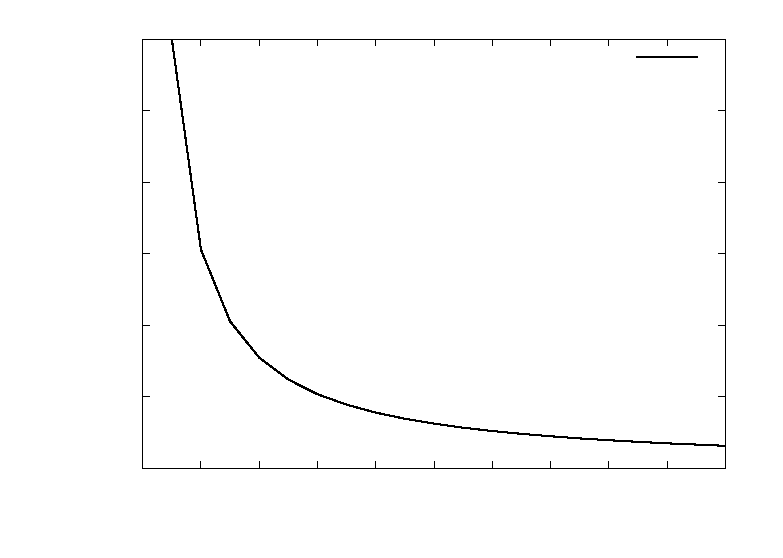
\includegraphics{./Graphics/nb_segs_diff_L2_cste}}%
    \gplfronttext
  \end{picture}%
\endgroup


\question{15.1}{En quoi la discrétisation en $\mu$ influence t-elle les résultats ?}
\question{15.2}{En quoi la discrétisation en espace influence t-elle les résultats ?}
\question{16.1}{Implémenter dans le code l'accélération par diffusion synthétique.}
\question{16.2}{Répéter l'expérience de la question 14 ; que peut-on constater ?}
\question{17.1}{Remplacer le schéma ``diamant'' par un schéma ``upwind''.}
\question{17.2}{Reprendre la question 14 ; que peut-on constater ?}

% GNUPLOT: LaTeX picture with Postscript
\begingroup
  \makeatletter
  \providecommand\color[2][]{%
    \GenericError{(gnuplot) \space\space\space\@spaces}{%
      Package color not loaded in conjunction with
      terminal option `colourtext'%
    }{See the gnuplot documentation for explanation.%
    }{Either use 'blacktext' in gnuplot or load the package
      color.sty in LaTeX.}%
    \renewcommand\color[2][]{}%
  }%
  \providecommand\includegraphics[2][]{%
    \GenericError{(gnuplot) \space\space\space\@spaces}{%
      Package graphicx or graphics not loaded%
    }{See the gnuplot documentation for explanation.%
    }{The gnuplot epslatex terminal needs graphicx.sty or graphics.sty.}%
    \renewcommand\includegraphics[2][]{}%
  }%
  \providecommand\rotatebox[2]{#2}%
  \@ifundefined{ifGPcolor}{%
    \newif\ifGPcolor
    \GPcolorfalse
  }{}%
  \@ifundefined{ifGPblacktext}{%
    \newif\ifGPblacktext
    \GPblacktexttrue
  }{}%
  % define a \g@addto@macro without @ in the name:
  \let\gplgaddtomacro\g@addto@macro
  % define empty templates for all commands taking text:
  \gdef\gplbacktext{}%
  \gdef\gplfronttext{}%
  \makeatother
  \ifGPblacktext
    % no textcolor at all
    \def\colorrgb#1{}%
    \def\colorgray#1{}%
  \else
    % gray or color?
    \ifGPcolor
      \def\colorrgb#1{\color[rgb]{#1}}%
      \def\colorgray#1{\color[gray]{#1}}%
      \expandafter\def\csname LTw\endcsname{\color{white}}%
      \expandafter\def\csname LTb\endcsname{\color{black}}%
      \expandafter\def\csname LTa\endcsname{\color{black}}%
      \expandafter\def\csname LT0\endcsname{\color[rgb]{1,0,0}}%
      \expandafter\def\csname LT1\endcsname{\color[rgb]{0,1,0}}%
      \expandafter\def\csname LT2\endcsname{\color[rgb]{0,0,1}}%
      \expandafter\def\csname LT3\endcsname{\color[rgb]{1,0,1}}%
      \expandafter\def\csname LT4\endcsname{\color[rgb]{0,1,1}}%
      \expandafter\def\csname LT5\endcsname{\color[rgb]{1,1,0}}%
      \expandafter\def\csname LT6\endcsname{\color[rgb]{0,0,0}}%
      \expandafter\def\csname LT7\endcsname{\color[rgb]{1,0.3,0}}%
      \expandafter\def\csname LT8\endcsname{\color[rgb]{0.5,0.5,0.5}}%
    \else
      % gray
      \def\colorrgb#1{\color{black}}%
      \def\colorgray#1{\color[gray]{#1}}%
      \expandafter\def\csname LTw\endcsname{\color{white}}%
      \expandafter\def\csname LTb\endcsname{\color{black}}%
      \expandafter\def\csname LTa\endcsname{\color{black}}%
      \expandafter\def\csname LT0\endcsname{\color{black}}%
      \expandafter\def\csname LT1\endcsname{\color{black}}%
      \expandafter\def\csname LT2\endcsname{\color{black}}%
      \expandafter\def\csname LT3\endcsname{\color{black}}%
      \expandafter\def\csname LT4\endcsname{\color{black}}%
      \expandafter\def\csname LT5\endcsname{\color{black}}%
      \expandafter\def\csname LT6\endcsname{\color{black}}%
      \expandafter\def\csname LT7\endcsname{\color{black}}%
      \expandafter\def\csname LT8\endcsname{\color{black}}%
    \fi
  \fi
    \setlength{\unitlength}{0.0500bp}%
    \ifx\gptboxheight\undefined%
      \newlength{\gptboxheight}%
      \newlength{\gptboxwidth}%
      \newsavebox{\gptboxtext}%
    \fi%
    \setlength{\fboxrule}{0.5pt}%
    \setlength{\fboxsep}{1pt}%
\begin{picture}(7200.00,5040.00)%
    \gplgaddtomacro\gplbacktext{%
      \csname LTb\endcsname%%
      \put(946,704){\makebox(0,0)[r]{\strut{}$0.4$}}%
      \put(946,1116){\makebox(0,0)[r]{\strut{}$0.45$}}%
      \put(946,1527){\makebox(0,0)[r]{\strut{}$0.5$}}%
      \put(946,1939){\makebox(0,0)[r]{\strut{}$0.55$}}%
      \put(946,2350){\makebox(0,0)[r]{\strut{}$0.6$}}%
      \put(946,2762){\makebox(0,0)[r]{\strut{}$0.65$}}%
      \put(946,3173){\makebox(0,0)[r]{\strut{}$0.7$}}%
      \put(946,3585){\makebox(0,0)[r]{\strut{}$0.75$}}%
      \put(946,3996){\makebox(0,0)[r]{\strut{}$0.8$}}%
      \put(946,4408){\makebox(0,0)[r]{\strut{}$0.85$}}%
      \put(946,4819){\makebox(0,0)[r]{\strut{}$0.9$}}%
      \put(1078,484){\makebox(0,0){\strut{}$0$}}%
      \put(2223,484){\makebox(0,0){\strut{}$0.2$}}%
      \put(3368,484){\makebox(0,0){\strut{}$0.4$}}%
      \put(4513,484){\makebox(0,0){\strut{}$0.6$}}%
      \put(5658,484){\makebox(0,0){\strut{}$0.8$}}%
      \put(6803,484){\makebox(0,0){\strut{}$1$}}%
    }%
    \gplgaddtomacro\gplfronttext{%
      \csname LTb\endcsname%%
      \put(198,2761){\rotatebox{-270}{\makebox(0,0){\strut{}$Phi(x, mu)$}}}%
      \put(3940,154){\makebox(0,0){\strut{}$x}}%
      \csname LTb\endcsname%%
      \put(5816,4646){\makebox(0,0)[r]{\strut{}$N_{\mu}$=2}}%
      \csname LTb\endcsname%%
      \put(5816,4426){\makebox(0,0)[r]{\strut{}$N_{\mu}$=4}}%
      \csname LTb\endcsname%%
      \put(5816,4206){\makebox(0,0)[r]{\strut{}$N_{\mu}$=6}}%
      \csname LTb\endcsname%%
      \put(5816,3986){\makebox(0,0)[r]{\strut{}$N_{\mu}$=8}}%
      \csname LTb\endcsname%%
      \put(5816,3766){\makebox(0,0)[r]{\strut{}$N_{\mu}$=10}}%
      \csname LTb\endcsname%%
      \put(5816,3546){\makebox(0,0)[r]{\strut{}$N_{\mu}$=12}}%
      \csname LTb\endcsname%%
      \put(5816,3326){\makebox(0,0)[r]{\strut{}$N_{\mu}$=14}}%
      \csname LTb\endcsname%%
      \put(5816,3106){\makebox(0,0)[r]{\strut{}$N_{\mu}$=16}}%
    }%
    \gplbacktext
    \put(0,0){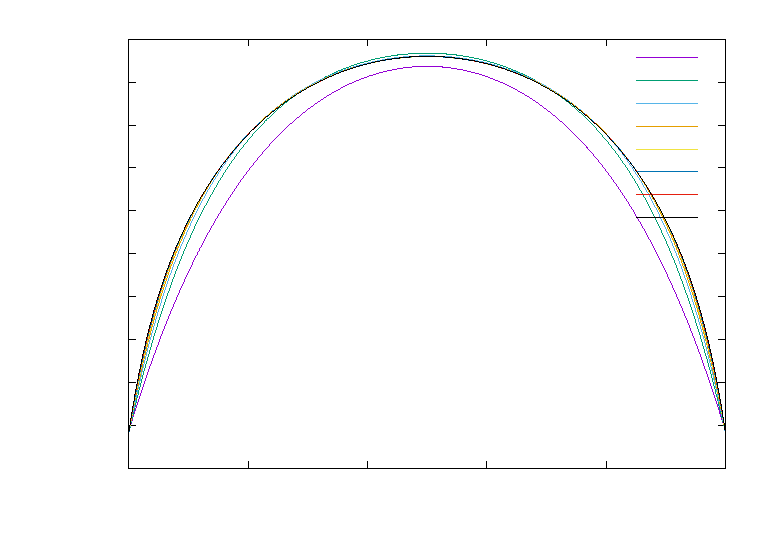
\includegraphics{.\loop_nb_pts_mu_cste}}%
    \gplfronttext
  \end{picture}%
\endgroup


\end{document}

%%% Local Variables:
%%% mode: latex
%%% TeX-master: t
%%% End:
